\documentclass[12pt,english,brazil,a4paper,utf8,oneside]{utfpr-tcc}

%Reviewing
\newcommand{\filipe}[1]{\textcolor{blue}{{\it [Filipe: #1]}}}
% copying from you, Filipe, hahaa
\newcommand{\daniel}[1]{\textcolor{red}{{\it [Daniel: #1]}}}

% carrega o arquivo configuracoes.tex que contém os pacotes e comandos Latex.
%
% Esse arquivo conterá pacotes e comandos utilizados na monografia
%
% Observação - devido a um erro do sharelatex foi necessário colocar na raiz do projeto os seguintes arquivos:
% gcnumparser.sty, fcprefix.sty, fmtcount.sty, fc-poruges.def, fcportuguese.def.
% Tal problema foi relatado em: https://github.com/nlct/fmtcount/issues/26
% Quando o sharelatex corrigir o problema acredito que podemos remover esses arquivos do projeto. At. Luiz Arthur.
%

% Este comando não é necessário: utilizei apenas para deixar o latex2rtf
% feliz (e descobrir a codificação do texto).
\usepackage[utf8]{inputenc}

% Suporte a figuras e subfiguras
\usepackage{graphics}
\usepackage{subfigure}

% Suporte a tabelas (principalmente do cronograma)
\usepackage{tabularx}
\usepackage{multirow}
\usepackage{array}
\usepackage{tabularx}
\usepackage{colortbl}
\usepackage{hhline}
\usepackage{xcolor}


% better tables
\usepackage{booktabs}

% frame box
\usepackage{mdframed}

% Escalar fontes para redimencionar, por exemplo tabelas
\usepackage{scalefnt}

% Algoritmos.
\usepackage{algorithm,algorithmic}

\usepackage[alf]{abntex2cite}

% the table's styles
\usepackage{booktabs}

% Elementos geralmente utilizados na tabela do cronograma
\newcommand{\fullcell}{\multicolumn{1}{>{\columncolor[gray]{0.5}}c}{}}
\newcommand{\fullcellline}{\multicolumn{1}{>{\columncolor[gray]{0.5}}c|}{}}
\newcommand{\mc}[3]{\multicolumn{#1}{#2}{#3}}
\newcommand{\y}{\rule{8pt}{4pt}}
\newcommand{\n}{\hspace*{8pt}}

% Define o caminho das figuras
\graphicspath{{images/}}

%% Configuração de glossário
\usepackage[portuguese]{nomencl}
\usepackage[nogroupskip,acronym,nomain,nonumberlist,nopostdot,nohypertypes={acronym}]{glossaries}

\makenoidxglossaries

% para siglas em português
\newcommand{\sigla}[2]
{
 \newglossaryentry{#1}{
  name=#1,
  description={#2},
  first={#2 (#1)},
  long={#2}
 }  
}

% para siglas de língua estrangeira, nessas a descrição longa fica em itálico.
\newcommand{\siglaIt}[2]
{
 \newglossaryentry{#1}{
  name=#1,
  description={\textit{#2}},
  first={\textit{#2} ({#1})},
  long={\textit{#2}}
 }  
}

% --- Estilos para apresentação de Código ----- %
\usepackage{listings}
\lstset{escapechar=§}
\lstloadaspects{formats}

\lstset{
	aboveskip=0cm,
	stringstyle=\ttfamily,
	showstringspaces = false,
	basicstyle=\scriptsize\ttfamily,
	commentstyle=\color{gray!45},
	keywordstyle=\bfseries,
	ndkeywordstyle=\bfseries,
	identifierstyle=\ttfamily,
	numbers=left,
	numbersep=15pt,
	numberstyle=\tiny,
	numberfirstline = false,
	breaklines=true
}

\lstdefinelanguage{JavaScript}{
	keywords={typeof, new, true, false, catch, function, return, null, catch, switch, var, const, let, async, await, if, in, while, do, else, case, break, from},
	ndkeywords={class, export, boolean, throw, implements, import, this},
	sensitive=false,
	comment=[l]{//},
	morecomment=[s]{/*}{*/},
	morestring=[b]',
	morestring=[b]"
}

% Diff language
\usepackage{xcolor}
\definecolor{diffstart}{named}{lightgray}
\definecolor{diffincl}{named}{blue}
\definecolor{diffrem}{named}{red}

\lstset{
	aboveskip=0cm,
	stringstyle=\scriptsize,
	showstringspaces = false,
	basicstyle=\scriptsize\ttfamily,
	commentstyle=\color{gray!45},
	keywordstyle=\bfseries,
	ndkeywordstyle=\bfseries,
	identifierstyle=\ttfamily,
	numbers=left,
	numbersep=15pt,
	numberstyle=\tiny,
	numberfirstline = false,
	breaklines=true
}

\lstdefinelanguage{diff}{
    basicstyle=\scriptsize\ttfamily,
	morecomment=[f][\color{diffstart}]{@@},
	morecomment=[f][\color{diffincl}]{+\ },
	morecomment=[f][\color{diffrem}]{-\ },
	morestring=[b]',
	morestring=[b]",
	keywords={typeof, new, true, false, catch, function, return, null, catch, switch, var, const, let, async, await, if, in, while, do, else, case, break, from},		
	ndkeywords={class, export, boolean, throw, implements, import, this},
}
% --- Fim da Definição de Estilos para apresentação de Código ----- %
% carrega o arquivo constantes.tex que contém dados do curso/monografia que NÃO DEVEM ser alterados. 
% Dados do curso que não precisam de alteração
\university{Universidade Tecnológica Federal do Paraná}
\universityen{Federal University of Technology -- Paraná}
\universityunit{Departamento Acadêmico de Computação}
\address{Campo Mourão}
\addressen{Campo Mourão, PR, Brazil}
\documenttype{Monografia}
\documenttypeen{Monograph}
\degreetype{Graduação}
% carrega o arquivo variaveis.tex que contém dados do acadêmico/monografia que DEVEM ser alterados.
% Dados do curso. Caso seja BCC:
\program{Curso de Bacharelado em Ciência da Computação}
\programen{Undergradute Program in Computer Science}
\degree{Bacharel}
\degreearea{Ciência da Computação}
% Caso seja TSI:
% \program{Curso Superior de Tecnologia em Sistemas para Internet}
% \programen{Undergradute Program in Tecnology for Internet Systems}
% \degree{Tecnólogo}
% \degreearea{Tecnologia em Sistemas para Internet}


% Dados da disciplina. Escolha uma das opções e a descomente:
% TCC1:
\goal{Proposta de Trabalho de Conclusão de Curso de Graduação}
\course{Trabalho de Conclusão de Curso 1}
% TCC2:
% \goal{Trabalho de Conclusão de Curso de graduação}
% \course{Trabalho de Conclusão de Curso 2}


% Dados do TCC (precisa alterar)
\author{Daniel Venturini}  % Seu nome
\title{Estudo empírico sobre \textit{Break change} no ecossistema do NPM} % Título do trabalho
\titleen{An Empirical Study of Breaking Changes in the npm Ecosystem } % Título traduzido para inglês
\advisor{Prof. Dr. Ivanilton Polato} % Nome do orientador. Lembre-se de prefixar com "Prof. Dr.", "Profª. Drª.", "Prof. Me." ou "Profª. Me."}
\coadvisor{Prof. Dr. Igor Scaliante Wiese} % Nome do coorientador, caso exista. Caso não exista, comente a linha.
\depositshortdate{2019} % Ano em que depositou este documento

% Dados da ficha catalografica. Ela é opcional, mas é uma boa ideia inserí-la. Exemplos para geração (http://fichacatalografica.sibi.ufrj.br/)
\fichacatautor{}  % Nome conforme citado (ou seja, no formato "Sobrenome, Nome").
\fichacatbib{Biblioteca da UTFPR de Campo Mourão} % Não alterar
\fichacatpum{M488} % Código Cutter-Sanborn. Use a primeira letra do sobrenome seguido do número conforme as primeiras letras do sobrenome e a tabela http://www.amormino.com.br/cutter-sanborn/cutter1.html
\fichacatpalcha{} % Assuntos do trabalho. Cada item deve ser enumerado e separado por ponto: 1. xxx. 2. yyy. 3. zzz.
\fichacatpdois{} % Deixar em branco

% carrega o arquivo listaabreviaturas.tex que está dentro do diretório pretextual, esse arquivo contém as siglas utilizadas na monografia.
% quando a sigla for de língua portuguesa utilize \sigla{SIGLA}{Significado em português}
% quando a sigla for de língua estrangeira utilize \siglaIt{SIGLA}{Significado em Inglês}

\siglaIt{NPM}{Node Package Manager}
\siglaIt{HTTP}{HyperText Transfer Protocol}
\siglaIt{API}{Application Programming Interface}

% No texto quando for utilizar a sigla utilize os seguintes comandos:
%\acrlong{label} - acronimo/sigla longo
%\acrshort{label} - acronimo/sigla curta
%\Gls{TCP} - sigla com o significado primeiro em Maiusculo
%\GLS{TCP} - sigla com o significado tudo em MAIUSCULO
%\gls{TCP} - sigla com o significado tudo em minusculo % usando glossaries

\begin{document}

\frontmatter
\maketitle

% Dedicatória é opcional, para usar descomentar a linha a seguir e edite o arquivo pretextual/dedicatoria.tex
%\dedicate{Para minha mãe, para meu pai e para você...} % Opcional - descomentar para usar

% Agradecimento é opcional, para usar descomentar a linha a seguir e edite o arquivo pretextual/dedicatoria.tex
%\begin{agradecimentos}

agradeço agradeço agradeço agradeço agradeço agradeço agradeço agradeço  agradeço agradeço agradeço agradeço agradeço agradeço agradeço agradeço agradeço agradeço agradeço agradeço agradeço agradeço agradeço agradeço agradeço agradeço agradeço agradeço agradeço agradeço agradeço agradeço agradeço agradeço agradeço agradeço agradeço agradeço agradeço agradeço agradeço agradeço agradeço agradeço agradeço agradeço agradeço agradeço agradeço agradeço agradeço agradeço agradeço agradeço agradeço agradeço agradeço agradeço agradeço agradeço agradeço agradeço agradeço agradeço agradeço agradeço agradeço agradeço agradeço agradeço agradeço agradeço 

\end{agradecimentos} % Opcional - descomentar para usar

% carrega o arquivo resumo.tex que está dentro do diretório pretextual, esse arquivo deve conter o resumo da monografia.
\begin{resumo}
%Elemento obrigatório, constituído de uma sequência de frases concisas e objetivas, em forma de texto.  Deve apresentar os objetivos, métodos empregados, resultados e conclusões.  O resumo deve ser redigido em parágrafo único, conter no máximo 500 palavras e ser seguido dos termos representativos do conteúdo do trabalho (palavras-chave).

% TODO: se possível, escreva um resumo estruturado. Para TCC 1, o resumo estruturado teria os seguintes elementos:
\textbf{Contexto:} o \textit{npm} é largamente utilizado e é o maior repositório para uma dada linguagem. Os pacotes hospedados no \textit{npm} dependem um dos outros, criando uma rede de interconectividade entre eles. Entretanto, os provedores evoluem independentemente dos seus clientes e, por vezes, introduzem alterações que podem causar um comportamento inesperado nos clientes. Essas alterações são as \textit{breaking changes} e se tornam um problema quando os clientes as recebem, mas não deveriam receber.\\
\textbf{Objetivo:} este trabalho propõe mensurar e categorizar as \textit{breaking changes} e analisar como os clientes se recuperam delas.\\
\textbf{Método:} de uma amostra dos pacotes do \textit{npm}, copiá-los localmente, resolver a versão dos seus provedores para a última versão disponível no momento da \textit{release} do cliente. Posteriormente, executar o pacote através dos \textit{scripts npm install/npm test}. Então, para cada \textit{release} do cliente que resultou em erro, verificar no código da \textit{release} e no repositório do provedor para confirmar se o erro foi causado pelo provedor, sendo então uma \textit{breaking change}.\\
% \textbf{Resultados esperados:} 
% ou, para TCC 2:
% \textbf{Contexto:} \\
% \textbf{Objetivo:} \\
% \textbf{Método:} \\
% \textbf{Resultados:} \\
% \textbf{Conclusões:}

% Palavras-chaves, separadas por ponto (tente não definir mais do que cinco)
\palavraschaves{\textit{npm}. \textit{Breaking change}. Versionamento Semântico. Dependências}
\end{resumo}
% carrega o arquivo abstract.tex que está dentro do diretório pretextual, esse arquivo deve conter um resumo escrito na linguá inglesa para a monografia.
%% Caso seja TCC 2, precisa traduzir o resumo e as palavras-chaves para inglês:
\begin{abstract}
PUT THE ABSTRACT HERE...

% \textbf{Context:}
% \textbf{Objective:}
% \textbf{Method:}
% \textbf{Results:}
% \textbf{Conclusions:}

% Palavras-chaves em inglês, separadas por ponto.
% \keywords{}
\end{abstract}

% Listas (opcionais, mas recomenda-se a partir de 5 elementos)
\listoffigures
\listoftables
%\listofacronyms
\printnoidxglossaries

% Sumário
\tableofcontents

\mainmatter

% Capítulos da monografia:
\chapter{Introdução}
\label{cap:introducao}

O \textit{Node Package Manager} (\textit{npm}) é um gerenciador de pacotes para o \textit{Node.js} que possui um \textit{website}\footnote{https://npmjs.org}, no qual se pode consultar os pacotes, e um registro\footnote{http://registry.npmjs.org/}, no qual os pacotes publicados são armazenados. Lançado em 2009, seu principal objetivo é facilitar o compartilhamento de códigos escritos em \textit{JavaScript} -- além de outras linguagens de programação. Atualmente, o \textit{npm} ocupa a posição de maior repositório\daniel{ou registro?} para uma dada linguagem, com mais de 1 milhão de pacotes.\footnote{http://www.modulecounts.com} O \textit{npm} é um dos que impulsionaram o \textit{JavaScript} a se tornar um ecossistema completo, com pacotes, \textit{frameworks}, aplicativos \textit{mobiles}, aplicativos \textit{web} entre outros \cite{introduction:npm} e também,  97\% dos aplicativos \textit{web} são oriundos do \textit{npm}.\footnote{https://blog.npmjs.org/post/180868064080/this-year-in-javascript-2018-in-review-and-npms}

O \textit{npm} estimula o compartilhamento de código entre os pacotes e, por causa disso, contém o maior número de dependências entre os pacotes \cite{teorical_reference:npm_2}. Nesse cenário, o termo cliente refere-se àquele pacote que depende de outro pacote para executar, e o termo provedor refere-se àquele pacote que provê recursos para os seus cliente, conforme definidos na Seção \ref{ref-teo:prov_clie}. Assim, como muitos pacotes estão dependendo mutuamente, há uma rede que interconecta os pacotes, e quando há um erro em algum provedor, um grande número de clientes podem ser afetados. Foi exatamente isso que ocorreu através de um 


pacote chamado \textit{left-pad}.\footnote{https://blog.npmjs.org/post/141577284765/kik-left-pad-and-npm} Esse pacote foi removido do \textit{npm} por seu desenvolvedor e impactou milhares de outros pacotes em apenas 2.5 horas, incluindo pacotes renomados como o \textit{babel}\footnote{https://github.com/babel/babel} e o \textit{atom}\footnote{https://github.com/atom/atom} que propagaram essa quebra de dependência para seus clientes. Assim, problemas de comunicação entre os pacotes realmente ocorrem no ecossistema do \textit{npm} e por isso esse foi escolhido como estudo de caso, devido à rede de interconectividade entre os pacotes.

Um defeito que causa problemas de comunicações entre os pacotes são as \textit{breaking changes}, descritas na Seção \ref{ref-teo:breaking_change}. Uma \textit{breaking change} é uma alteração no provedor que o torna incompatível com as suas versões anteriores \cite{intro:break_change}, fazendo com que seus clientes tenham um comportamento indesejado. Um exemplo de \textit{breaking change} ocorreu na \textit{release optipng@0.2.0} na qual o método \textit{OptiPng.getBinaryPath} foi renomado para \textit{OptiPng.getBinPath}.\footnote{https://github.com/papandreou/node-optipng/compare/v0.1.1...v0.2.0\#diff-366460cd3c3170c9c84340631e6f8e4fL22-R19} Porém, o método foi renomeado por engano e a \textit{release} errônea foi publicada em uma versão \textit{minor} -- nível de versão do Versionamento Semântico, especificado na Seção \ref{ref-teo:semver} --, fazendo com que todos os clientes que tinham acesso àquele método não tivesse mais. Assim, o código \ref{cod:bc:optipng} executa normalmente com o \textit{optipng@0.1.1}, mas ao atualizar para o \textit{optipng@0.2.0}, esse código sofre uma \textit{breaking change} -- o que não deveria acontecer com uma \textit{release minor}.

\begin{lstlisting}[style=Javascript, label=cod:bc:optipng, caption={Código que sofre \textit{breaking change} do \textit{optipng}}]
var OptiPng = require('optipng');
var cb = {apply: () => {}};
OptiPng.getBinaryPath(cb);
\end{lstlisting}

Apesar de ser um erro facilmente detectável, esse foi consertado somente após 34 dias, conforme mostra a Figura \ref{fig:bc_optipng}. Esta correção foi realizada em um \textit{commit}\footnote{https://github.com/papandreou/node-optipng/commit/a155f2b078224be18367847bbcbd3df3c379deea} no qual o desenvolvedor comentou que a renomeação do método ocorreu por engano.

\begin{figure}
    \centering
    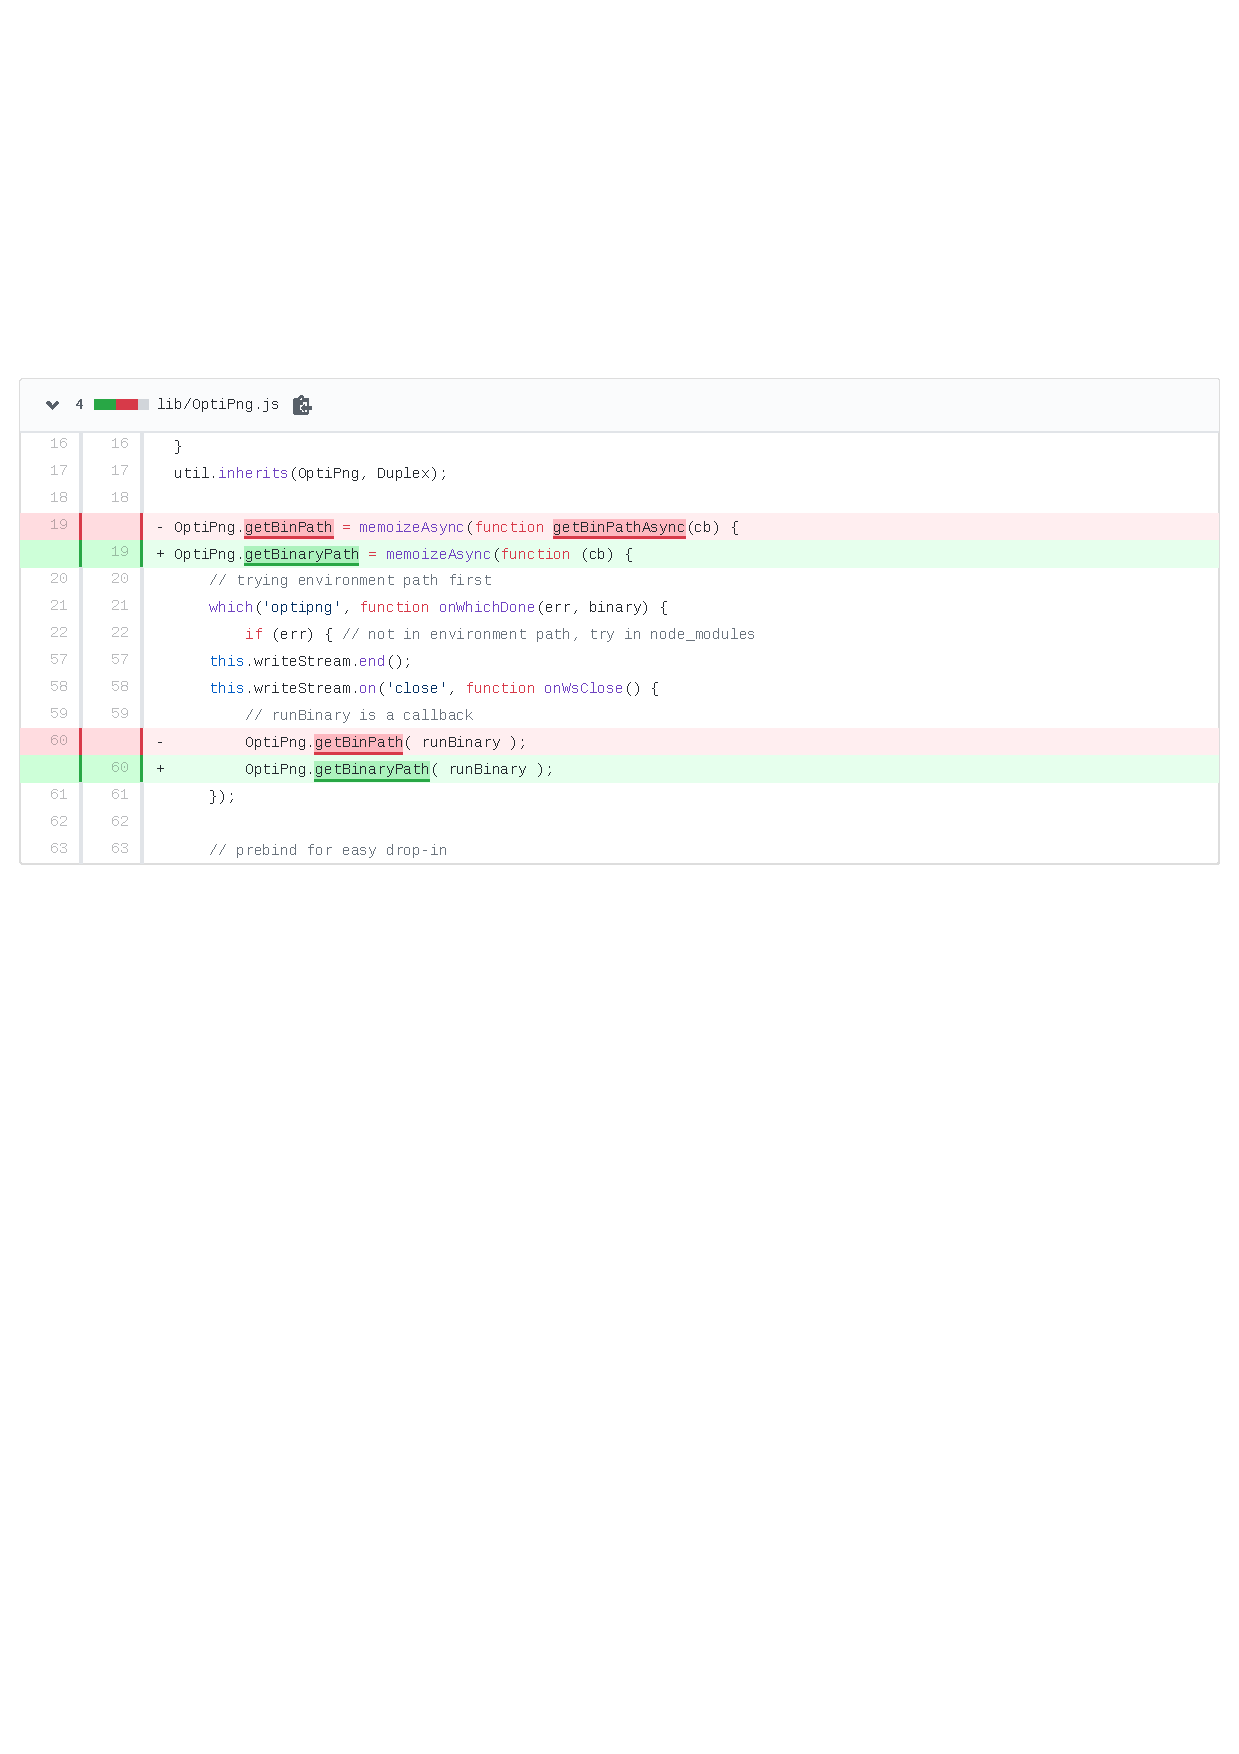
\includegraphics[scale=0.65]{figuras/bc_example.pdf}
    \caption{\textit{Commit} que corrigiu a \textit{breaking change}}
    \label{fig:bc_optipng}
\end{figure}{}

Alterações no código que causam \textit{breaking change} devem ser introduzidas em \textit{releases} versionadas com o incremento do nível \textit{major}, seguindo as especificações do Versionamento Semântico, definidos na Seção \ref{ref-teo:semver}. Assim, um cliente pode especificar se deseja ou não receber as \textit{releases} que contêm \textit{breaking change}. Entretanto, pesquisas relacionadas mostram que as \textit{breaking changes} são introduzidas erroneamente pelos provedores, assim, impactando os clientes. \citeonline{teorical_reference:bc_1} constatou que 9\% das \textit{releases} dos três pacotes com mais dependentes no \textit{npm} introduziram \textit{breaking changes} indevidamente e \citeonline{noregrets2018} apresentou uma ferramenta para detecção de \textit{breaking changes} e também constatou que 9\% das \textit{releases} introduziram \textit{breaking changes} quando não deveriam introduzir.
\daniel{Esses são os que eu coloquei nos trabalhos relacionados}

Além de quantificar as \textit{breaking changes} no ecossistema do \textit{npm}, este trabalho apresenta uma proposta para categorizar essas \textit{breaking changes} e verificar como os clientes se recuperam. Para isso, foi utilizado uma amostra representativa dos clientes no \textit{npm} e, para cada uma de suas \textit{releases}, foi verificado se houve alteração nas \textit{releases} que os clientes aceitavam dos provedores. Então, as versões dos provedores foram resolvidas para a última versão disponível até momento da publicação da \textit{release} do cliente e as \textit{releases} foram executadas através dos \textit{scripts npm install/npm test}. Após, foi feita uma análise manual no código das \textit{releases} que resultaram em erro para confirmar se o erro se tratava de uma \textit{breaking change} ou não. Por fim, foi feita uma análise nos repositórios dos provedores que introduziram as \textit{breaking change} para recuperar informações, tais como, tipo de \textit{breaking change}, tempo que levou até ser consertada, o nível da versão que a \textit{breaking change} foi introduzida/consertada.

Desse modo, o Capítulo \ref{cap:ref-teorico} contém a descrição de todos os termos utilizados ao longo desse trabalho. O Capítulo \ref{cap:qp} contém a motivação e o método para cada uma das questões de pesquisa. O Capítulo \ref{cap:metodologia} descreve sobre a manipulação dos dados que serão utilizados nessa pesquisa\daniel{serão ou foram?}. Por fim, o Capítulo \ref{cap:cronograma} apresenta o cronograma previsto das atividades faltantes para terminar esse trabalho.

% isso estava nos results
%\filipe{o erro sempre se manifesta no cliente, acho que o lance é que você consegue identificar se o erro foi proveniente de uma chamada a uma função do provedor ou do próprio cliente (ou algum outro provedor que não interessa à análise).}

%\filipe{breaking change (defeito no provedor) vs. manifestação da breaking change (manifestação do defeito do provedor no cliente)}
\chapter{Referencial Teórico}
\label{cap:ref-teorico}
Neste capítulo está descrito os fundamentos pertinentes a este trabalho. A Seção \ref{ref-teo:npm} apresenta o conceito e o funcionamento do \gls{npm} bem como a questão das dependências. A Seção \ref{ref-teo:prov_clie} distingue os termos \textit{provedor} e \textit{cliente}. Também para diferenciar termos, a Seção \ref{ref-teo:pac_rel_ver} discorre sobre \textit{pacote}, \textit{release} e \textit{versão}. A Seção \ref{ref-teo:semver} explica o que é \textit{Versionamento Semântico} e o \textit{SemVer} e como eles são utilizados no ecossistema do \gls{npm}. Porfim, a Seção \ref{ref-teo:breaking_change} conceitua e exemplifica as \textit{breaking changes}.

\section{\gls{npm}}
\label{ref-teo:npm}
O \gls{npm} é um gerenciador de pacotes para o \textit{Node.js}. Lançado em 2009, seu principal objetivo é facilitar o compartilhamento de códigos escritos em \textit{Javascript}. Atualmente, o \gls{npm} ocupa a posição de maior repositório para uma dada linguagem, com mais de 1 milhão de projetos\footnote{http://www.modulecounts.com/}. O \gls{npm} permite que, com apenas um simples comando, o usuário realize o download, publique, instale e desinstale pacotes diretamente de vários repositórios. A facilidade proporcionada pelo \gls{npm} corrobora para a grande popularidade do \textit{Javascript} e para que o compartilhamento de bibliotecas seja largamente utilizado, uma vez que 97\% dos aplicativos \textit{web} são oriundos do \textit{NPM}\footnote{https://blog.npmjs.org/post/180868064080/this-year-in-javascript-2018-in-review-and-npms}.

O ecossistema \gls{npm} estimula o compartilhamento de código entre aos pacotes. Por causa disso, dentre os demais repositórios, o \gls{npm} contém a maior distribuição de dependência entre os pacotes \cite{teorical_reference:npm_2}. Dessa maneira, como muitos pacotes estão dependendo mutuamente uns dos outros, há uma gigantesca rede de interconectividade entre os pacotes e, quando há um erro qualquer em algum desses pacotes, um grande número de outros pacotes podem ser afetados. Foi exatamente isso que ocorreu com um pacote chamado \textit{left-pad}\footnote{https://blog.npmjs.org/post/141577284765/kik-left-pad-and-npm}. Esse pacote foi removido do \textit{NPM} por seu desenvolvedor e impactou milhares de pacotes em apenas 2.5 horas, incluindo pacotes renomados como o \textit{babel}\footnote{https://github.com/babel/babel} e o \textit{atom}\footnote{https://github.com/atom/atom} que, devido ao grande número de dependentes, cascatearam o erro para inúmeros outros pacotes.
%In fact, 97\% of the code in a modern web application comes from npm

\section{Provedor e Cliente}
\label{ref-teo:prov_clie}
O pacote provedor é aquele que provê recursos ao pacote cliente, ou seja, contém interfaces públicas para acesso às suas funcionalidades. O termo \textit{pacote provedor} pode ser interpretado como \textit{bibliotecas} ou \textit{dependências}. Por exemplo, quando é executado o seguinte comando

\begin{lstlisting}[style=bash, label=cod:install:provider]
npm install mocha
\end{lstlisting}
o \gls{npm} salva o \textit{mocha} no \textit{package.json} como um provedor. Assim, o pacote \textit{mocha} é um provedor direto, pois foi instalado diretamente pelo usuário. Entretanto, as dependências do \textit{mocha} também são instaladas, mas de forma indireta pelo \gls{npm}. Estes outros pacotes são chamados de \textit{provedores indiretos}, pois não dependem que o usuário instale-os diretamente com o comando \textit{npm install}. A Figura \ref{fig:provider} mostra que, através do comando \textit{npm ls}, o pacote \textit{mocha} é um provedor direto do \textit{client}, pois o \textit{client} requer o \textit{mocha} para executar. Já o pacote \textit{glob} é um provedor direto do \textit{mocha}, e um provedor indireto do pacote \textit{client}.

\begin{figure}
    \centering
    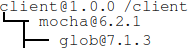
\includegraphics{figuras/provider_directly_undirectly.png}
    \caption{\textit{mocha} como provedor direto e \textit{glob} como indireto do \textit{client}}
    \label{fig:provider}
\end{figure}{}

Já o pacote cliente é aquele que está acessando as interfaces públicas do provedor. Quando uma \textit{break change} é introduzida pelo provedor -- direto ou indireto --, é sempre no pacote cliente que esta \textit{break change} se manifesta, causando o encerramento da execução. O pacote cliente é aquele que possui a responsabilidade de atualizar a versão de seus provedores no \textit{package.json} quando esses publicam uma \textit{release} com correções, enquanto que o pacote provedor possui a responsabilidade de indicar o nível de compatibilidade que sua nova \textit{release} está introduzindo \cite{teorical_reference:semver}.

\section{Pacote, \textit{Release} e Versão}
\label{ref-teo:pac_rel_ver}
Neste trabalho, a palavra \textit{pacote} refere-se a um \textit{software} hospedado no \gls{npm}. Esse \textit{software} contém seu nome, seus arquivos e suas versões. Por exemplo, quando nos referimos ao pacote \textit{mocha}, nos referimos à ideia genérica desse pacote, sem levar em consideração uma versão específica ou seu estado em algum instante, mas sim, apenas ao pacote como um todo.

Já a palavra \textit{release} designa o estado de um pacote em um determinado instante. Uma \textit{release} é denotada por uma versão específica desse pacote, isto é, um conjunto de arquivos distintos das demais \textit{releases}. Cada \textit{release} é acompanhada da publicação de uma nova versão do pacote no \gls{npm}.

Por fim, o termo \textit{versão} é utilizado para especificar e distinguir um determinado estado de uma \textit{release}. Uma \textit{versão} é uma \textit{string} no padrão \textit{SemVer} que identifica unicamente uma determinada \textit{release} e é utilizada pelo \gls{npm} no arquivo \textit{package.json} para especificar um \textit{range} de versões que o cliente aceita.

\section{Versionamento Semântico e \textit{SemVer}}
\label{ref-teo:semver}
O Versionamento Semântico\footnote{https://semver.org} é um padrão para versionamento de \textit{releases} de um projeto que considera o tipo de alteração introduzida na \textit{release}. As regras do Versionamento Semântico foram idealizadas por Tom Preston-Werner -- criador do \textit{GitHub} -- que incentiva todos os desenvolvedores à utilizarem este padrão, uma vez que as regras são baseadas em práticas comuns já utilizadas em projetos \cite{teorical_reference:semver}. Uma \textit{string} de versão no padrão do Versionamento Semântico possui os níveis \textit{<MAJOR>.<MINOR>.<PATCH>}\footnote{a \textit{string} pode ser estendida para versões \textit{beta, alpha, pre}, entre outros, tal como \textit{x.y.z-beta.0}}, que devem ser incrementados, quando o desenvolvedor publicar uma \textit{release}, de acordo com o seguinte critério:

\begin{itemize}
    \item \textit{MAJOR}: deve ser incrementado quando a \textit{release} introduz \textit{breaking changes};
    \item \textit{MINOR}: incrementado quando for adicionado melhorias/novas funcionalidades que mantenham a compatibilidade com as \textit{releases} anteriores; e
    \item \textit{PATCH}: deve ser incrementado quando a \textit{release} contém correção de \textit{bugs}.
\end{itemize}{}

Dessa maneira, se um projeto contém a sua última \textit{release} versionada como \textit{2.1.0}, por exemplo, o seu nível \textit{major} é o 2; o \textit{minor}, 1; e o \textit{patch}, 0. Ao publicar uma nova \textit{release}, se essa conter uma \textit{breaking change}, então deverá ser publicada com a versão \textit{3.0.0}; se for introduzida uma nova funcionalidade, \textit{2.2.0}; se houver uma correção de \textit{bugs}, \textit{2.1.1}.

O \textit{SemVer} é uma \textit{string} de versionamento que especifica um intervalo de versões, ou \textit{range}. Com o \textit{SemVer} é possível especificar quais são as \textit{releases} que o cliente aceita do seu provedor. Há vários padrões de \textit{range}\footnote{https://github.com/npm/node-semver\#ranges} especificados pelo \textit{SemVer}, mas os mais comuns, utilizados pelo \gls{npm}, são:

\begin{itemize}
    \item \textit{X-Ranges (*)}: este \textit{range} especifica para o \gls{npm} que o cliente aceita qualquer nova \textit{release} do provedor, até mesmo as \textit{releases} com \textit{breaking changes};
    \item \textit{Caret Ranges (\textasciicircum)}: este é o \textit{range} mais comum e o padrão do \gls{npm}. Com o \textit{Caret Range}, o cliente especifica que o \gls{npm} só deve descarregar novas \textit{releases} do provedor que contenham novas funcionalidades e correções de erros, mas que não contenham \textit{breaking changes}, ou seja, o cliente aceita todas as \textit{releases} das quais foram atualizadas os níveis \textit{patch} ou \textit{minor};
    \item \textit{Tilde Ranges (\textasciitilde)}: neste \textit{range}, o cliente especifica para o \textit{NPM} que somente as \textit{releases patch} do provedor são aceitas.
\end{itemize}{}

O \gls{npm} utiliza o padrão \textit{SemVer} no arquivo \textit{package.json} -- arquivo de configuração do projeto que contém todas os provedores e suas respectivas versões. Ao executar o comando \textit{npm install express --save}, para instalar o provedor \textit{express}\footnote{https://www.npmjs.com/package/express} por exemplo, o \gls{npm} -- além de descarregar este provedor -- irá salvar no \textit{package.json} o nome do provedor com sua versão atual em modo \textit{range}, de acordo com a Figura \ref{fig:dep_express}.

\begin{figure}
    \centering
    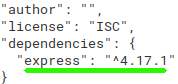
\includegraphics{figuras/dependencies_express.png}
    \caption{Modo como o \gls{npm} salva no \textit{package.json} a versão de uma dependência}
    \label{fig:dep_express}
\end{figure}{}

Com a informação do \textit{range} do provedor no \textit{package.json}, o cliente não precisa se preocupar com as novas atualizações de seus provedores, uma vez que o \gls{npm}, ao instalar novamente os provedores, sempre irá descarregar as \textit{releases} mais recentes que são aceitas pelo \textit{range SemVer}, especificado pelo cliente. Por padrão, o \gls{npm} especifica o \textit{Caret Range}, mas o cliente pode especificar outro \textit{range} manualmente no \textit{package.json} ou pode utilizar a opção \textit{--save-exact} para especificar a versão sem o \textit{range}, fazendo com que o \gls{npm} sempre instale esta versão específica.

\section{Breaking Change}
\label{ref-teo:breaking_change}
Uma \textit{break change} é uma alteração no pacote provedor que produz defeitos nos pacotes clientes \cite{teorical_reference:semver}. As \textit{break changes} surgem quando o pacote provedor, que previamente era executado com sucesso pelo cliente, publica uma \textit{release} que causa no cliente um comportamento inesperado, resultando em um erro. Durante o desenvolvimento de \textit{software}, os provedores precisam introduzir \textit{breaking changes}, pois quando só há \textit{releases} compatíveis com versões anteriores, o \textit{software} perde muitas oportunidades de evolução \cite{teorical_reference:bc_2}. Desta maneira, as \textit{break changes} são importantes para a evolução de um \textit{software}, uma vez que apenas \textit{releases} retro-compatíveis podem estagnar o \textit{software} limitando sua evolução. Assim, as \textit{breaking changes} também são sinônimos de evolução. Exemplo disso é o \textit{Node.js} que publica uma \textit{release} incrementando o nível \textit{major} a cada 6 meses\footnote{https://github.com/nodejs/node\#release-types}. Desta maneira, introduzir \textit{breaking changes} em níveis \textit{major} permite que os \textit{softwares} evoluam sem manter-se preso à versões anteriores.

Para evitar que os impactos de uma \textit{break change} afetem os clientes, os provedores publicam suas \textit{releases} com \textit{breaking changes} incrementando o nível \textit{major} da sua nova versão, seguindo a regra do Versionamento Semântico. Dessa maneira, os clientes de versões prévias que especificaram o provedor com o \textit{range caret} -- \textit{range} especificado por padrão pelo \gls{npm} -- ou o \textit{range tilde} não serão afetados por uma \textit{break change}. Porém, uma \textit{breaking change} pode ser introduzida em uma \textit{release} intencionalmente -- quando é atualizada o nível \textit{major} --, mas também pode ser introduzida inesperadamente -- quando é atualizado os níveis \textit{minor} ou \textit{patch}. Dessa maneira, o problema das \textit{breaking changes} está no fato do desenvolvedor introduzi-las em \textit{releases minor} ou \textit{patch}, resultando em defeitos nos clientes, uma vez que o cliente irá receber essa \textit{release} que contenha \textit{break changes} -- desde que o \textit{range} especificado para a versão do provedor aceite esta \textit{release} --, e se o cliente não espera ou não tratou previamente essa \textit{break change}, com certeza sua execução estará comprometida.

Um exemplo de \textit{breaking change} ocorreu na \textit{release optipng@0.2.0}: a \gls{API} \textit{OptiPng.getBinaryPath} foi renomada para \textit{OptiPng.getBinPath}\footnote{https://github.com/papandreou/node-optipng/pull/6}. Porém, a \gls{API} foi renomeada por engano e a \textit{release} errônea foi publicada em uma versão \textit{minor}, fazendo com que todos os clientes que tinham acesso àquela \gls{API} não a tivesse mais. Assim, o código \ref{cod:bc:optipng} executa normalmente com o \textit{optipng@0.1.1}, mas ao atualizar para o \textit{optipng@0.2.0}, este código sofre uma \textit{breaking change} -- o que não deveria acontecer com uma \textit{release minor}  -- conforme mostra a Figura \ref{fig:bc_optipng} (a).

\begin{lstlisting}[style=Javascript, label=cod:bc:optipng, caption={Código que sofre \textit{breaking change} do \textit{optipng}}]
var OptiPng = require('optipng');
var cb = {apply: () => {}};
OptiPng.getBinaryPath(cb);
\end{lstlisting}

Apesar de ser um erro facilmente detectável, esse foi consertado após 34 dias. E esta correção foi realizada em um \textit{commit}\footnote{https://github.com/papandreou/node-optipng/commit/a155f2b078224be18367847bbcbd3df3c379deea} no qual o desenvolvedor informou no comentário que a renomeação da \gls{API} ocorreu por engano, conforme a Figura \ref{fig:bc_optipng} (b), quando o desenvolvedor desfez a renomeação.

\begin{figure}
    \centering
    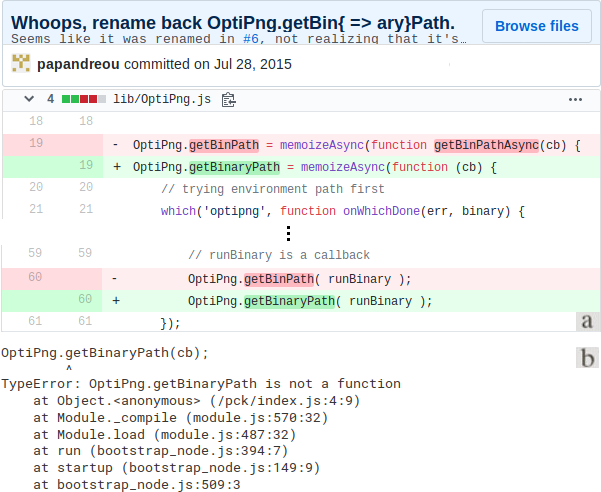
\includegraphics[scale=0.65]{figuras/bc_optipng.png}
    \caption{\textit{a}: \textit{stack trace} da \textit{break change}. \textit{b}: \textit{commit} que corrigiu a \textit{break change}}
    \label{fig:bc_optipng}
\end{figure}{}

\subsection{Casos de \textit{non-break changes}}
Além de alterações que resultam em \textit{breaking changes}, há algumas alterações que são causadas por provedores mas que, nessa pesquisa, não serão consideradas como \textit{breaking changes}. Essas alterações são:

\begin{itemize}
    \item Alterações da versão do \textit{Node.js}: o \textit{Node.js} atualizou o seu nível \textit{major} de \textit{0.x} para \textit{7.x} em apenas 3 anos\footnote{https://nodejs.org/en/download/releases}, mas isso não significa que os pacotes evoluíram seus códigos sempre para a última \textit{release} do \textit{Node.js}, e o inverso é valido, ou seja, os pacotes podem ter evoluído seus códigos na mesma frequência do \textit{Node.js}. Por exemplo, considere um pacote cliente executando no \textit{Node.js 0.x} com um provedor que evoluiu seu código para a sintaxe do \textit{Node.js 6.x}, que não é aceita no \textit{Node.js 0.x}. Desta maneira, não há uma versão do \textit{Node.js}  na qual seja possível executar o pacote cliente sem que no provedor seja manifestado um erro. Assim, erros nos provedores ocasionados por versões do \textit{Node.js} não serão considerados como \textit{break changes}, pois o erro foi causado pelo \textit{Node.js}, que não reconhece a sintaxe, e não pelo provedor;
    \item Exclusão de uma \textit{release}/\textit{provedor} do \gls{npm}: pelas regras do \gls{npm}, uma \textit{release} só pode ser removida até 72 horas após ter sido publicada\footnote{https://docs.npmjs.com/cli/unpublish\#description}. Entretanto, quando uma \textit{release} é removida do \gls{npm} e o cliente especificou aquela \textit{release}, isso gera um erro no \textit{script install}. Assim, o erro é causado pelo \gls{npm} que não consegue encontrar a \textit{release}, e não pelo provedor. No caso do provedor ter sido removido do \gls{npm} o caso é o mesmo: um provedor só pode ser removido após 72 horas. Entretanto, anterior ao acontecimento do \textit{left-pad}, os pacotes -- e \textit{releases} também -- podiam ser removidos do \gls{npm} em qualquer circunstância. Por isso, quando um pacote removido do \gls{npm} causar um erro, não será considerado como uma \textit{break change}.
    \item Alterações em serviços externos: os pacotes podem fazer uso de sistemas externos, tais como acesso à \textit{API}'s de sites e sistemas, e recuperar dados desses. Entretanto, ao longo do tempo, naturalmente, essas \textit{API}'s podem alterar seus dados, o que gera inconsistências em seus clientes. Mas esse tipo de erro não é considerado como uma \textit{break change}; e
    \item Cliente aceita \textit{releases} major do provedor: quando o cliente especifica em seu \textit{package.json} que aceita qualquer \textit{release} do provedor, através de um \textit{X-range}, o cliente então está aceitando \textit{releases} que foram introduzidas \textit{break changes}. Por isso, quando um cliente for impactado por uma \textit{break change} no provedor, e que foi corretamente introduzida em uma \textit{release major}, então o problema está no cliente que aceitou a \textit{break change} mas não a tratou.
\end{itemize}{}

\section{Trabalhos Relacionados}
\label{sec:related_works} % Esse capítulo e nome é apenas uma sugestão.
%% ATENÇÃO - veja com o seu orientador se você vai ter este capítulo e se este vai ter nome!
\chapter{Trabalhos Relacionados}
\label{cap:trabalhos:relacionados}

Apresente aqui os trabalhos similares ao seu trabalho ou que são importantes para o entendimento do seu trabalho...

(ATENÇÃO - veja com o seu orientador se você vai ter este capítulo e se este vai ter nome!)

\section{Uso de citações}
\label{cap:trabalhos:sec:relacionados:uso:citacoes}

Este é um exemplo do uso de citações no texto \cite{tomasulo:algorithm:5392028}.

Segundo \citeonline[p.~56]{Moore:2000:CMC:333067.333074} para citações textuais...

De acordo com o trabalho de \citeonline{Moore:2000:CMC:333067.333074} para citações textuais não tão específicas...


TEXTO TEXTO TEXTO TEXTO TEXTO TEXTO TEXTO TEXTO TEXTO TEXTO TEXTO TEXTO TEXTO TEXTO TEXTO TEXTO TEXTO TEXTO TEXTO TEXTO TEXTO TEXTO TEXTO TEXTO TEXTO TEXTO TEXTO TEXTO TEXTO TEXTO TEXTO TEXTO TEXTO TEXTO TEXTO TEXTO TEXTO TEXTO TEXTO TEXTO TEXTO TEXTO TEXTO TEXTO TEXTO TEXTO TEXTO TEXTO TEXTO TEXTO TEXTO TEXTO TEXTO TEXTO TEXTO TEXTO TEXTO TEXTO TEXTO TEXTO TEXTO TEXTO TEXTO TEXTO TEXTO TEXTO TEXTO TEXTO TEXTO TEXTO TEXTO TEXTO TEXTO TEXTO TEXTO TEXTO TEXTO TEXTO TEXTO TEXTO TEXTO TEXTO TEXTO TEXTO TEXTO TEXTO TEXTO TEXTO TEXTO TEXTO TEXTO TEXTO TEXTO TEXTO TEXTO TEXTO TEXTO TEXTO TEXTO TEXTO TEXTO TEXTO TEXTO TEXTO TEXTO TEXTO TEXTO TEXTO TEXTO TEXTO TEXTO TEXTO TEXTO TEXTO TEXTO TEXTO TEXTO TEXTO TEXTO TEXTO TEXTO TEXTO TEXTO TEXTO TEXTO TEXTO TEXTO TEXTO TEXTO TEXTO TEXTO TEXTO

%---------------------------------------------------%
\section{Considerações Finais}
\label{cap:trabalhos:relacionados:sec:consideracoes:finais}

Esta é uma sugestão de seção para dar um fechamento em cada uma dos capítulos.

(ATENÇÃO - veja com o seu orientador se é uma seção necessária (pois trate-se de estilo de escrita)) % Esse capítulo e nome é apenas uma sugestão.
%% ATENÇÃO - veja com o seu orientador se você vai ter este capítulo e se este vai ter nome!
\chapter{Proposta}
\label{cap:proposta}

Esse capítulo é mais indicado para TCC 1, no qual o aluno pode expor melhor qual é a proposta de seus trabalho para a realização do TCC 1 e 2. Bem como o cronograma para realização das atividades.

(ATENÇÃO - veja com o seu orientador se você vai ter este capítulo e se este vai ter nome!)

TEXTO TEXTO TEXTO TEXTO TEXTO TEXTO TEXTO TEXTO TEXTO TEXTO TEXTO TEXTO TEXTO TEXTO TEXTO TEXTO TEXTO TEXTO TEXTO TEXTO TEXTO TEXTO TEXTO TEXTO TEXTO TEXTO TEXTO TEXTO TEXTO TEXTO TEXTO TEXTO TEXTO TEXTO TEXTO TEXTO TEXTO TEXTO TEXTO TEXTO TEXTO TEXTO TEXTO TEXTO TEXTO TEXTO TEXTO TEXTO TEXTO TEXTO TEXTO TEXTO TEXTO TEXTO TEXTO TEXTO TEXTO TEXTO TEXTO TEXTO TEXTO TEXTO TEXTO TEXTO TEXTO TEXTO TEXTO TEXTO TEXTO TEXTO TEXTO TEXTO TEXTO TEXTO TEXTO TEXTO TEXTO TEXTO TEXTO TEXTO TEXTO TEXTO TEXTO TEXTO TEXTO TEXTO TEXTO TEXTO TEXTO TEXTO TEXTO TEXTO TEXTO TEXTO TEXTO TEXTO TEXTO TEXTO TEXTO TEXTO TEXTO TEXTO TEXTO TEXTO TEXTO TEXTO TEXTO TEXTO TEXTO TEXTO TEXTO TEXTO TEXTO TEXTO TEXTO TEXTO TEXTO TEXTO TEXTO TEXTO TEXTO TEXTO TEXTO TEXTO TEXTO TEXTO TEXTO TEXTO TEXTO TEXTO TEXTO TEXTO

%---------------------------------------------------%
\section{Cronograma de Atividades}
\label{cap:proposta:sec:cronograma}

(ATENÇÃO - Esta é apenas uma sugestão de elaboração de cronograma, veja com seu orientador!)

Em TCC 1 talvez seja interessante apresentar uma cronograma de realização das atividades da proposta que englobe as atividades do TCC 2.

Nesta seção são apresentadas as atividades a serem desenvolvidas para a execução da proposta. O cronograma de realização das tarefas é apresentado na Tabela~\ref{tab:cronograma}.

\begin{enumerate}
\item \textbf{Escrita do Projeto TCC 1.}
\item \textbf{Estudo de Técnicas...}
\item \textbf{Implementação da Ferramenta ...}
\item \textbf{Testes com o conjunto de \textit{benchmarks}.}
\item \textbf{Estudo de técnicas de Escalonamento de Tarefas.}
\item \textbf{Entrega do TCC 1}
\item \textbf{Apresentação do TCC 1}
\item \textbf{Realização de Experimentos.}
\item \textbf{Atividade do TCC 2}
\item \textbf{Escrita do TCC2}
\item \textbf{Entrega do TCC 2.}
\item \textbf{Apresentação do TCC 2.}
\end{enumerate}

\begin{table}[h!]
\renewcommand{\arraystretch}{1.3}
\caption{Cronograma de atividades}
\label{tab:cronograma}
\scalefont{0.9}
\begin{tabular}{|c|c|c|c|c|c|c|c|c|c|c|c|c|}
\hline
\multirow{2}{*}{\textbf{\textbf{Atividade}}} & \multicolumn{4}{c|}{\textbf{2014}}& \multicolumn{8}{c|}{\textbf{2015}} \\ \cline{2-13} 
& \multicolumn{1}{l|}{\textbf{Set}} & \multicolumn{1}{l|}{\textbf{Out}} & \multicolumn{1}{l|}{\textbf{Nov}} & \multicolumn{1}{l|}{\textbf{Dez}} & \multicolumn{1}{l|}{\textbf{Jan}} & \multicolumn{1}{l|}{\textbf{Fev}} & \multicolumn{1}{l|}{\textbf{Mar}} & \multicolumn{1}{l|}{\textbf{Abr}} & \multicolumn{1}{l|}{\textbf{Mai}} & \multicolumn{1}{l|}{\textbf{Jun}} & \multicolumn{1}{l|}{\textbf{Jul}} & \multicolumn{1}{l|}{\textbf{Ago}} \\ \hline
\textbf{1}  & X &   &   &   &   &   &   &   &   &   &   &  \\ \hline
\textbf{2}  & X & X & X & X &   &   &   &   &   &   &   &  \\ \hline
\textbf{3}  &   & X & X & X & X & X &   &   &   &   &   &  \\ \hline
\textbf{4}  &   &   & X & X & X & X &   & X & X &   &   &  \\ \hline
\textbf{5}  &   &   & X & X & X &   &   &   &   &   &   &  \\ \hline
\textbf{6}  &   &   & X & X & X & X & X & X & X & X &   &  \\ \hline
\textbf{7}  &   &   & X & X &   & X & X &   & X & X &   &  \\ \hline
\textbf{8}  &   &   &   & X & X &   & X & X &   & X & X &  \\ \hline
\textbf{9}  &   &   &   &   & X & X & X & X & X & X & X & X \\ \hline
\textbf{10} &   &   &   &   &   &   &   &   &   &   &   & X \\ \hline
\end{tabular}
\end{table}

%---------------------------------------------------%
\section{Considerações Finais}
\label{cap:proposta:consideracoes:finais}

Esta é uma sugestão de seção para dar um fechamento em cada uma dos capítulos.

(ATENÇÃO - veja com o seu orientador se é uma seção necessária (pois trate-se de estilo de escrita)) % Esse capítulo e nome é apenas uma sugestão (bom para TCC 1).
\chapter{Questões de Pesquisa}
\label{cap:qp}

Este trabalho propõe um estudo sobre as \textit{breaking changes} e seus impactos no ecossistema do \gls{npm}. Para isso, três questões de pesquisa foram desenvolvidas para que seja possível executar o estudo. A seguir, há a motivação para cada questão de pesquisa. Nesta Seção estão descritos os métodos utilizados para responder cada uma das questões de pesquisa.

\section{QP1. Com que frequência \textit{breaking changes} impactam nos pacotes clientes?}
\label{sec:qp1}

\subsubsection{Motivação}
\label{sec:qp1:motivation}
No ecossistema do \gls{npm}, uma \textit{release} que contenha um erro pode afetar uma grande quantidade de pacotes, uma vez que a rede de dependências do npm é relativamente densa \cite{teorical_reference:npm_2}. Para evitar que \textit{breaking changes} se manifestem nos pacotes clientes, os provedores introduzem as \textit{breaking changes} em \textit{releases major}, seguindo o padrão do Versionamento Semântico, e os clientes podem utilizar \textit{strings semver} para aceitar apenas as versões \textit{minor} e \textit{patch} dos provedores -- o que é o padrão do \gls{npm}. Entretanto, nem sempre o provedor é capaz de distinguir se suas alterações são ou não \textit{breaking changes} \cite{noregrets2018}, ou, muitas vezes, as \textit{breaking changes} são introduzidas sem que o provedores percebam. Portanto, quando as \textit{breaking changes} são introduzidas em \textit{releases minor} ou \textit{patch}, elas podem causar comportamentos inesperados no cliente. Nesta RQ, será quantificado as manifestações das \textit{breaking changes} nos pacotes clientes. Assim, entender a frequência que os provedores publicam \textit{breaking changes} que afetam os clientes pode ajudar os clientes a tomar melhores decisões sobre como e quando atualizar a versão do seu provedor.

\subsubsection{Método}
\label{sec:qp1:approach}

Quando os comandos \textit{npm install} e \textit{npm test} resultam em erro, o \gls{npm} exibe o erro e todas as chamadas de funções, incluindo as invocações para os provedores em um \textit{stack trace}. O \textit{stack trace} é utilizado pelo \gls{npm} para apresentar informações sobre um determinado erro. A Figura \ref{fig:trace} mostra um exemplo genérico de um \textit{stack trace} exibido pelo \gls{npm}. Nessa Figura, no topo do \textit{stack trace}, contém o tipo do erro que interrompeu a execução do pacote cliente e a sua mensagem. Nas linhas abaixo, há todas as funções e arquivos que foram executados até a manifestação do erro. Com todos estes dados, o \textit{stack trace} foi a base para o rastreamento de cada erro, uma vez que ele foi utilizado para detectar as \textit{breaking changes}, pois através do \textit{stack trace} foi possível identificar com exatidão se o erro foi proveniente de uma chamada a uma função do provedor ou do próprio cliente.

\begin{figure}
    \centering
    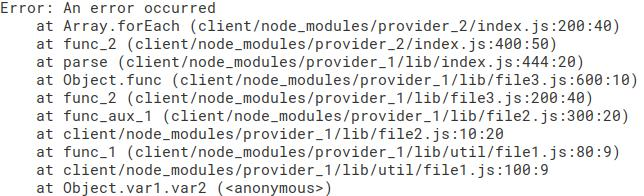
\includegraphics[scale=0.7]{figuras/stack_trace.jpeg}
    \caption{\textit{stack-trace} genérico}
    \label{fig:trace}
\end{figure}{}

Para quantificar as \textit{breaking changes}, foi necessário diferenciar entre um erro que foi causado pelo próprio pacote cliente, no qual não houve influência de nenhum provedor, e um erro que foi causado por algum dos provedores, sendo assim uma \textit{breaking change}. Esta diferenciação é necessária pois um determinado erro pode ter ocorrido no código do cliente e não em um provedor, assim não sendo um caso de \textit{breaking change}. Para realizar esta diferenciação, foram utilizadas as seguintes heurísticas:

\begin{itemize}
    \item Quando não houve registro de execução de uma função do provedor no \textit{stack trace}, o erro ocorreu no código do cliente e, a não ser que a execução resultou em erro por causa de um objeto retornado por algum provedor, o erro não foi causado por uma \textit{breaking change}. Assim, foi realizado alterações no código do cliente, tal como adições de \textit{console.log()}, para rastrear o erro;
    \item Quando houve registro de execução de uma função do provedor no \textit{stack trace}, o erro provavelmente se tratava de uma \textit{breaking change}. Então foi recuperado os nomes dos provedores e foram aplicados os próximos métodos para descobrir se o provedor -- e qual -- realmente causou o erro.

    \item \textit{Commits} realizados pelos clientes: foi verificado no \textit{GitHub} se o cliente tentou consertar algum erro após a \textit{release} que apresentou o erro. Se foi encontrado algum \textit{commit} com correções, foram feitas estas alterações no código do cliente para verificar se as modificações encontradas no \textit{GitHub} realmente refletiam a correção do erro. Assim, se as alterações apenas no código do cliente refletiam na correção do erro, sem que haja influência dos provedores, então o erro não se tratava de uma \textit{breaking change};

    \item Sistemas integrados ao \textit{GitHub}: alguns sistemas integrados ao \textit{GitHub} auxiliaram na investigação. Esses sistemas são o \textit{Travis\footnote{https://travis-ci.org}, Codeship\footnote{https://codeship.com}} entre outros, que armazenam os resultados da execução do pacote para cada \textit{commit}. Eles foram utilizados da seguinte maneira: se nesses sistemas integrados, a execução no \textit{commit} da \textit{release} do cliente foi realizado com sucesso e, ao executá-lo nesta pesquisa, resultou em erro, então esse caso evidencia a ocorrência de uma \textit{breaking change}, uma vez que o código do cliente estava na mesma \textit{working tree} do \textit{commit}. Mas, se a execução do cliente no momento do \textit{commit} resultou em erro, provavelmente os próximos \textit{commits} contêm alguma informação sobre o erro e sua correção, uma vez que esses sistemas integrados avisaram os desenvolvedores sobre o erro na execução.
    
    \begin{figure}
        \centering
        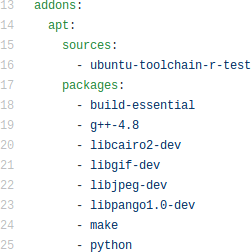
\includegraphics[scale=0.6]{figuras/false_positive.png}
        \caption{\textit{Script} requerido para executar com sucesso o pacote \textit{node-qrious}}
        \label{fig:false-positive}
    \end{figure}{}

    Em particular, o \textit{Travis} desempenhou um papel fundamental para identificar os erros, em especial, os falso-positivos -- casos que resultaram em erro, mas não eram. Um exemplo de falso-positivo ocorreu no pacote \textit{node-qrious}\footnote{https://www.npmjs.com/package/node-qrious}, que resultou em erro na execução, mas na análise manual, através do arquivo \textit{.travis.yml}\footnote{https://github.com/neocotic/node-qrious/blob/176ea348b9e51a8c1f0c5e2caa6cd4b0320ea5e2/.travis.yml} -- arquivo de configuração para o sistema integrado -- foi descoberto que o pacote requeria bibliotecas terceiras que, ao serem instaladas, resultou em sucesso na execução do pacote, conforme a Figura \ref{fig:false-positive}.
\end{itemize}{}

Portanto, cada erro foi analisado manualmente, com alterações no código do cliente, para certificar se o erro era um falso-positivo, um erro interno, uma \textit{non-breaking change} ou uma \textit{breaking change}. Essa separação foi importante para esta e para as próximas questões de pesquisa. Com isso, foi possível quantificar os casos \textit{breaking changes} por pacotes e por \textit{releases}.


\section{QP2. Como os pacotes provedores introduzem \textit{breaking changes} em uma \textit{release}?}
\label{sec:qp2}

\subsubsection{Motivação}
\label{sec:qp2:motivation}
Pesquisas anteriores apresentam estudos sobre \textit{breaking changes} no ecossistema do \gls{npm}. Entretanto, pelo fato do \textit{Javascript} ser dinâmico, esses estudos focaram apenas nas alterações de \gls{API}, tais como as remoções/renomeações, alterações na lista de parâmetros e alterações no tipo de retorno. Esses estudos foram realizados por  \citeonline{teorical_reference:bc_1} e \citeonline{noregrets2018} e não verificaram \textit{breaking changes} além das relacionadas às \gls{API}. Dessa maneira, além das alterações em \gls{API}, não se tem informações sobre como os provedores introduzem \textit{breaking changes}, ou seja, quais os principais casos que fazem com que o cliente sofra uma \textit{breaking changes}. Por causa da falta de informação, muitas \textit{breaking changes} são introduzidas, mas poderiam ser facilmente evitadas. Por isso, dimensionar e categorizar as \textit{breaking changes} ajudará os desenvolvedores a atentar-se para as \textit{breaking changes} mais comuns e tentar evitá-las, assim produzindo códigos menos favoráveis às \textit{breaking changes}.

\subsubsection{Método}
\label{sec:qp2:approach}
O objetivo da análise manual é descobrir o motivo que originou uma \textit{breaking changes}, ou seja, qual foi a alteração que o provedor realizou que causou a \textit{breaking change}, para que seja possível agrupa-las por suas similaridades. Porque o \textit{stack trace} sempre apresenta o erro de uma maneira genérica, às vezes, a mensagem de erro pode induzir a interpretação errônea do real motivo que originou a falha. Assim, o melhor local para se investigar quais foram as alterações que o provedor realizou é o \textit{GitHub}, no qual várias técnicas foram utilizadas para recuperar as informações necessárias:

\begin{itemize}
    \item Arquivos de alterações: os arquivos de registros de alterações, comumente nomeados por \textit{CHANGELOG.md} ou \textit{HISTORY.md}, contêm as descrições das principais alterações em cada \textit{releases} do projeto. Através da versão do provedor que foi descarregada do \gls{npm}, foi verificado nos arquivos de alterações quais foram as modificações introduzidas pelos provedores e se algumas dessas alterações diz respeito ao erro encontrado no cliente. Uma das informações mais relevantes nestes arquivos são as descrições de \textit{breaking changes}. Por exemplo, a versão \textit{5.0.0} do pacote \textit{Mocha} contém uma \textit{breaking change} que foi documentada no \textit{CHANGELOG.md}\footnote{https://github.com/mochajs/mocha/blob/master/CHANGELOG.md\#500--2018-01-17} de acordo com a Figura \ref{fig:bc_documentation} (a). Outro tipo de documentação equivalente são as \textit{releases-notes}, como pode ser visualizado na Figura \ref{fig:bc_documentation} (b) como o pacote \textit{wpxml2md} documentou \textit{breaking changes} nas \textit{releases-notes}\footnote{https://github.com/akabekobeko/npm-wpxml2md/releases/tag/v2.0.0}. Entretanto, apenas 46\% dos repositórios utilizados nesta pesquisa contêm algum dos dois registros.

    \item \textit{Issues/Pull-requests}: uma vez que uma \textit{breaking change} se manifesta em algum cliente, ele pode -- e deve -- registrar este erro através de uma \textit{issue} no repositório do provedor. O proveito de buscar informações nas \textit{issues} é que essas contêm comentários dos provedores e da comunidade, assim, há muitas informações sobre um determinado erro, além de várias outras \textit{issues} lincadas, ampliando a busca por informações. Da mesma maneira os \textit{pull-requests} foram utilizados para buscar informações sobre as \textit{breaking changes}.

    \item Versões prévias dos provedores: um ponto muito importante foi a instalação de versões prévias dos provedores. Uma vez que foi identificado qual provedor está causando a \textit{breaking change}, a instalação de outras versões ajudaram a descobrir a partir de qual \textit{release} do provedor a \textit{breaking change} foi introduzida, ou a partir de qual \textit{release} ela foi consertada. Com isso, as \textit{breaking change} ficaram mais fáceis de serem identificadas pois, uma vez que foi localizada a \textit{release} que introduziu o erro, pôde ser utilizado ferramentas de \textit{diff} para analisar o código introduzido e removido daquela determinada \textit{release} do provedor.

    \item Ferramentas de \textit{diff}: o uso da ferramenta que realizam o  \textit{diff} entre duas \textit{releases} de um pacote foi muito importante. Foi utilizado a ferramenta \textit{npm-diff}\footnote{https://github.com/danielventurini/npm-diff} e a ferramenta \textit{compare}\footnote{https://github.com/danielventurini/cnlg/compare/1.1.0..1.1.1} do \textit{GitHub}. Com isso, foi possível verificar o que foi adicionado e removido do código do provedor -- até mesmo do cliente -- em um determinado intervalo de versões. Assim, conhecendo exatamente o que foi introduzido e removido em uma determinada \textit{release}, torna-se mais fácil categorizar o tipo de alteração.
\end{itemize}

\begin{figure}
    \centering
    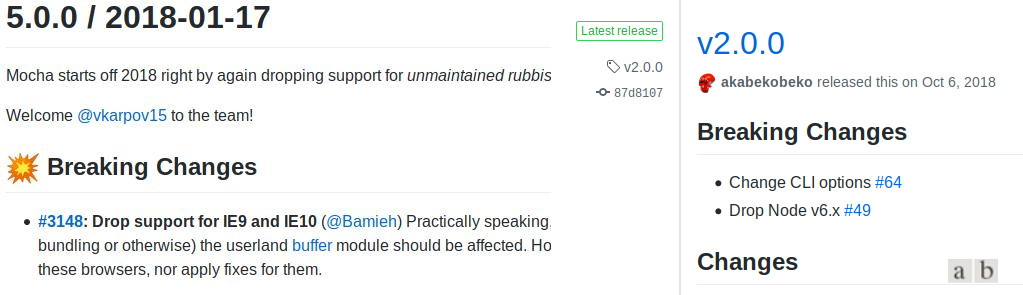
\includegraphics[scale=0.45]{figuras/bc_documentation.jpeg}
    \caption{Documentação de uma \textit{breaking change} no \textit{CHANGELOG} e nas \textit{release-notes}}
    \label{fig:bc_documentation}
\end{figure}{}

Após descobrir as alterações que introduziram uma \textit{breaking change}, categorias foram criadas para agrupar as \textit{breaking changes}. Por exemplo, quando um erro tratava-se de uma alteração de \gls{API}, uma categoria chamada \textit{Função Renomeada} foi criada e as demais \textit{breaking changes} que possuem características comuns a essa também foram categorizadas como \textit{Função Renomeada}. Assim será possível quantificar cada uma das categorias e visualizar as mais comuns. E o mesmo processo foi realizado para as demais \textit{breaking changes}, sempre visando criar categorias da maneira mais genérica que agrupassem os erros semelhantes.

Então, para todas as \textit{releases} analisadas manualmente, foram salvas as seguintes informações para que fosse possível quantificar as \textit{breaking changes} e responder esta e colaborar com as demais questões de pesquisa:

\begin{enumerate}
    \item Em que local o erro foi documentado: \textit{issue, changelog, pull-request} etc;
    \item Quem consertou o erro: cliente ou providor;
    \item Em qual nível do \textit{SEMVER} o erro foi reparado;
    \item Quanto tempo o erro levou até ser corrigido; e
    \item Por quantas \textit{releases} o erro persistiu.
\end{enumerate}{}

%---------------------------------------------------%

\section{QP3. Como os pacotes clientes se recuperam das \textit{breaking changes}?}
\label{sec:qp3}

\subsubsection{Motivação}
\label{sec:qp3:motivation}

Uma vez que uma \textit{breaking changes} é introduzida, o cliente deve se recuperar dessa, ajustando o seu próprio código. Isso se faz necessário pois, no ecossistema do  \gls{npm}, no qual centenas de milhares de pacotes estão conectados, uma simples \textit{release} com erro pode ocasionar na quebra de muitos clientes. No entanto, como os provedores evoluem independentemente dos clientes, erros e vulnerabilidades são difíceis de rastrear e corrigir nos clientes. Mesmo quando as vulnerabilidades podem ser corrigidas com a atualização para uma versão mais recente do provedor, pode haver incompatibilidades de \textit{API} -- entre outras incompatibilidades -- com os clientes que deve ser resolvido manualmente \cite{Foo:2018:ESC:3236024.3275535}. Dessa maneira, entender como os clientes reagem às \textit{breaking changes} ajudará os próprios clientes a conhecerem as alternativas frente às \textit{breaking changes} para que eles possam se recuperar da maneira mais eficiente.

\subsubsection{Método}
\label{sec:qp3:approach}
Uma vez que os clientes se recuperaram de um erro, há duas maneiras para se obter informações sobre esta recuperação. A primeira maneira é quando o provedor corrige seu código e o cliente apenas atualiza sua \textit{string} de versionamento no \textit{package.json}. Para o provedor consertar o erro, deve haver uma \textit{issue} no seu repositório. A segunda maneira é quando o próprio cliente conserta o código. Neste caso, o cliente pode corrigir o código do provedor e realizar um \textit{pull-request}. Também, o cliente pode alterar apenas o seu código para que execute normalmente com a \textit{release} do provedor que introduziu a \textit{breaking change}.

Todas as informações sobre esta questão de pesquisa foram recuperadas do \textit{GitHub}. As informações foram encontradas em \textit{CHANGELOGs, release-notes, issues} e \textit{pull-requests}. Os \textit{CHANGELOGs} contêm informações sobre os erros consertados. A partir das \textit{issues} é possível entender com os comentários dos clientes quais foram as ações que eles realizaram para se recuperar de uma determinada \textit{breaking change}. Pois, assim como o código de um pacote fica emaranhado com o código no restante do ecossistema ao qual ele pertence, o mesmo acontece com as \textit{issues}. Uma manifestação disso é que muitas \textit{issues} abertas em um projeto são vinculadas a \textit{issues} relacionadas, em projetos iguais ou diferentes, pois os desenvolvedores estão rastreando as causas de um problema \cite{Zhang:2018:WIL:3242887.3242891}. De maneira análoga, os \textit{pull-requests} que são relacionados ao mesmo problema também são marcados. Todas estas informações corroboram para descobrir como a \textit{breaking change} foi tratada/consertada e quem -- cliente ou provedor -- a consertou, caso tenha sido consertada.

Os \textit{commits} são alternativas para as \textit{issues} quando a busca se dá no repositório do cliente. Sobre os \textit{commits}, mensagens do tipo \textit{update dependencies, fix dependencies, fix errors} etc. sugerem que algum provedor foi atualizado para consertar algum erro ou um erro foi consertado diretamente no código do cliente. Estas informações são muito importantes, uma vez que o provedor corrigiu a \textit{breaking change} e o cliente apenas o atualizou. Assim, as mensagens dos \textit{commits} auxiliaram para descobrir os reais motivos da atualização -- ou retrocesso da versão. % Esse capítulo e nome é apenas uma sugestão.
% ATENÇÃO - veja com o seu orientador se você vai ter este capítulo e se este vai ter nome!
\chapter{Metodologia}
\label{cap:metodologia}

\begin{itemize}
    \item RQ1: How often do breaking changes manifest in the client package?
\end{itemize}

A stack trace is a report that provides information about program subroutines. It is commonly used for certain kinds of debugging, where a stack trace can help software engineers figure out where a problem lies or how various subroutines work together during execution. When \textit{npm install} or \textit{npm test} results in an error, it raises a stack trace. All information about the error and the calls to providers are shown in the stack trace. Figure \ref{fig:trace} shows a generic example of a stack trace of one error.

\begin{figure}
    \centering
    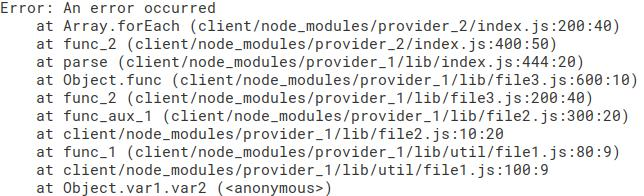
\includegraphics[scale=0.7]{figuras/stack_trace.jpeg}
    \caption{Generic stack-trace}
    \label{fig:trace}
\end{figure}{}

The stack trace is the base to analyze and an error.
All releases of any package that broke in the \textit{npm install} or \textit{npm test} were analyzed manually. The first step to analyze an error is differentiated between an error that wasn't caused by any provider, which is an error that occurred exclusively in the client package where the providers didn’t influence, and a breaking change error, that the errors occurred in provider package and it broke a client. There are two ways to conduct this step.

The first way is to take a look at the stack trace of the error and verify the calls to providers. When in the stack trace there isn't called to any providers, the error probably doesn’t refer a breaking change, because any provider was called in this error. So, the error is in the client code. To confirm this, the next commit in GitHub, after the release of the client, is verified. The objective is to verify if the error was fixed in any client commit. If true, the error is confirmed as a non-breaking change.
Some types of errors can be resolved in the code of the client. This error isn’t breaking change. Errors like \textit{SyntaxError} and \textit{ReferenceError}, where the client wrote the wrong code. Example:

\begin{lstlisting}[style=Javascript, label=cod:syntax:error, caption={Reference Error code in JavaScript}]
const a = 0 = 0;
\end{lstlisting}


In these errors, the npm raises a \textit{ReferenceError}. If the error is in the client code, nor is it necessary to look at \textit{GitHub}, because, for sure, the error is a non-breaking change. So, the code was fixed and the \textit{npm install} or \textit{npm test} is executed again to verify if any other error appeared.

The second way is when the errors can be a breaking change. This often occurs when the stack trace contains calls to any providers. However, providers like \textit{Mocha, Istanbul, Jasmine} and so on, that is, test frameworks, and task runners, like \textit{Grunt}, it is shown in stack trace but usually has no errors, because they only execute the files to test/tasks. So, when one of these providers is at the bottom of the stack tracer, they just called/execute the files/providers that contain the errors. Then, there’s a high probability that this error is a breaking change and this error can be caused by any provider.
To confirm this, the best place is in the \textit{GitHub}. The repository of the package contains all the information about the development. There are many ways to retrieve information. The easiest and most reliable way is to verify in a changelog file. These files, in general, are the \textit{CHANGELOG.md}, \textit{HISTORY.md} and others like this. These files contain the description of all changes about all packages releases. And many breaking changes are described there. For example, the release 5.0.0 of \textit{Mocha} contains a breaking change and was documented in \textit{CHANGELOG.md}. Figure \ref{fig:bc_documentation} show this documentation.

\begin{figure}
    \centering
    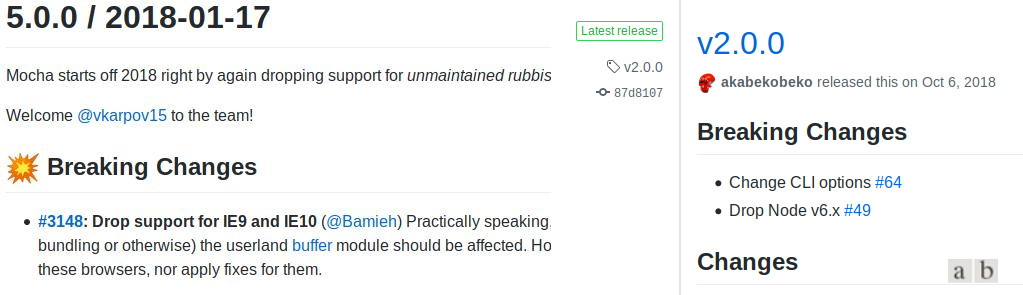
\includegraphics[scale=0.55]{figuras/bc_documentation.jpeg}
    \caption{Breaking Change documentation in README}
    \label{fig:bc_documentation}
\end{figure}{}

Other types of changelogs are the release notes. These are found in the comments of release. However, many and many repositories don’t contain a changelog file. Then, the next step is the search for any issue that contains some information about the error. In general, the issues contain much information, because of the developers and the owners of the package comment about the error. And more, many related issues are linked, increasing the number of information. Also, pull request works in the same way as issues.

Another important way is to install another release of the provider. So, it's possible to find out from which release the error started or which release the error was fixed. Also, there are other ways to verify if the error is in the provider. This is, compare the diff code between two provider releases; verify the provider commits; and change provider code.
The Figure \ref{fig:step_analyze} show a summary of these steps.

\begin{figure}
    \centering
    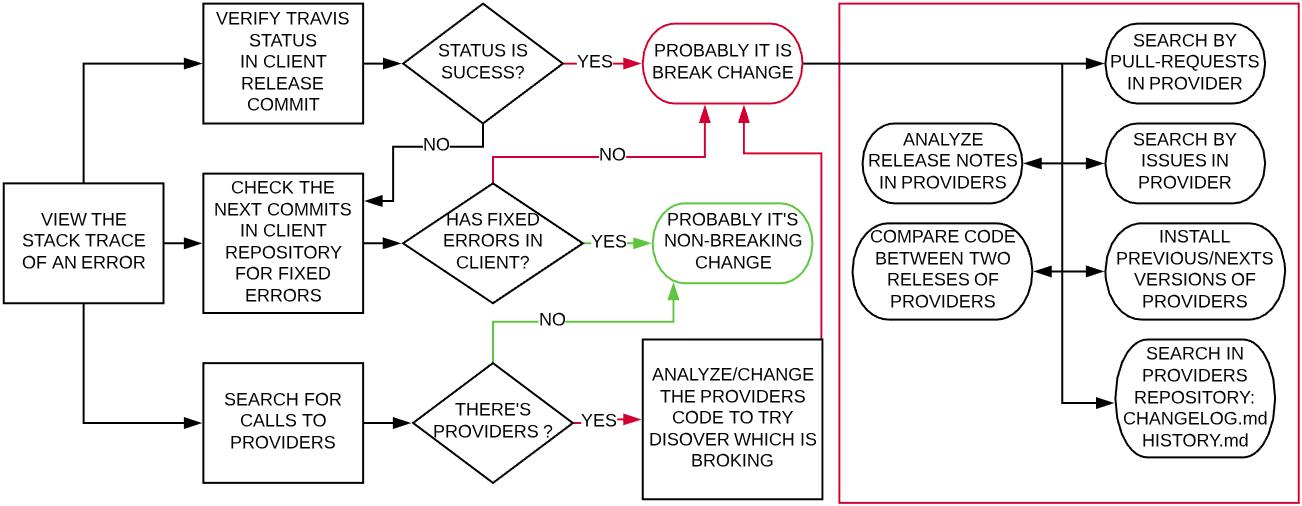
\includegraphics[scale=0.35]{figuras/step_analyze.jpeg}
    \caption{Steps to analyze an error}
    \label{fig:step_analyze}
\end{figure}
Some integrated systems can help to discover breaking changes. These systems are \textit{Travis, Jenkins, Codeship, CircleCI} and so on, and store the results of the npm install and npm test in the moment of a commit. It can help in the following way: if in the commit of a release the status of npm install or npm test was a success, and now is an error, then it occurred by a provider because the code of client is the same in the working tree and only the provider code was updated. However, just some of the sorted packages contain an integrated system.

Another detail is the packages that connect with some type of service likes, \textit{MySql, CouchDB, Redis} and so on. From all 385 packages, x required one of these services. When the \textit{npm install} or \textit{npm test} raises an error because of the connection, in manual analyze the required services were ability and re-executed the package. So, if the error was persister because the connection, the package was classified was \textit{Undiscovered Error}.

So, from all release analyze was saved many informations:

\begin{enumerate}
    \item Documentation about the error: issue, changelog, pull-request and so on;
    \item Who fixed the error: client or provider;
    \item How long did the error take to get fixed;
    \item Fixed in major, minor or patch; and
    \item In how many releases the error existed.
\end{enumerate}{}

Nor all information may be recovered. For example, if an error wasn't fixed, then neither the client nor the provider repaired the error.

\begin{itemize}
    \item RQ2: What issues in the provider package cause the manifestation of a breaking change?
\end{itemize}

For each error in \textit{npm install} or \textit{npm test}, it was manually analyzed. The objective is to do a grouping of similar errors and categorize then. For example, Figure \ref{fig:error_category} shows two errors in which one a function was renamed and the client tries to access the previous name.

\begin{figure}[!h]
    \centering
    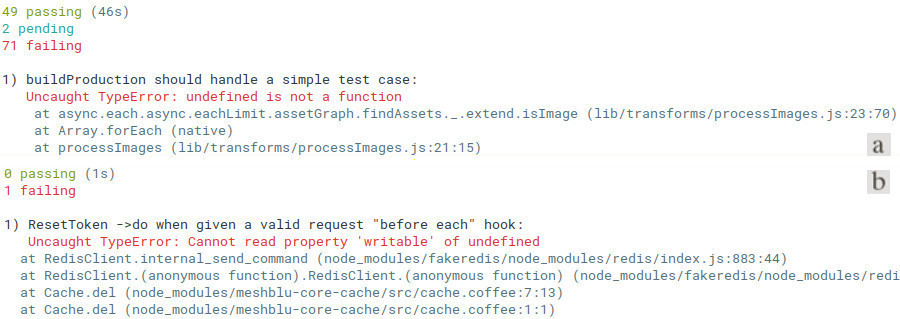
\includegraphics[scale=0.5]{figuras/error_category.jpeg}
    \caption{Two error caused by a renamed function}
    \label{fig:error_category}
\end{figure}

The first error in the Figure \ref{fig:error_category} is obvious: the client tries to access a variable like a function when it isn't a function. The second error talks about a property \textit{writable} that is access by an undefined object. There isn't any information about the function-related error, but, in manually analyze, it was observed that the provider change the name of a function. For this, in this code, the variable \textit{this.stream.writable} is undefined.

Once the provider causing the \textit{breaking change} has been discovered, there are several ways to find out the real reason that caused the error. These ways are described in Section \ref{cap:metodologia}. Then, all \textit{breaking changes} are classified based on his type.

\begin{itemize}
    \item RQ3: How do client packages recover from the manifestation of breaking change?
\end{itemize}

Since the customer recovers from the error, there are two ways to know how it recoverer. The first way is when the provider fixes his code and the client just updates the string of versioning in \textit{package.json}, if it needs. To the provider fixes the error, one issue may be done in his repository. The second way is when the client must do some work to fix the code. In this case, the client can fix the provider code and do a pull-request or change his code to work with the provider. And of course, may have cases that anyone does nothing. There is a breaking change and it’s never been fixed.

Where information about this RQ is retrieved is \textit{GitHub}. This information can be found at \textit{CHANGELOG, release-notes, issues,} and \textit{pull-requests}. If the \textit{changelog} contains information about fixed errors, in general, the related \textit{issues} are marked. From these \textit{issues}, a lot of more information can be recovered, like \textit{pull-requests} that are also marked in the \textit{issue}, other \textit{issues}, commentaries and more. All of this information can help us to discover which one -- client or provider -- fixed the \textit{breaking change} and how it was fixed.

\textit{Commits} are the alternative to \textit{issues} when the search is in the client repository. The \textit{commits} contain all changes in files and the all updates providers in \textit{package.json}. Commits message like \textit{update dependencies, fix dependencies, fix errors} an so on, suggests that something about any dependencies was fixed. This information is very important, because, since the provider was fixed and the client just updates it, the commit messages can tell the reason for this update - or downgrade.

%---------------------------------------------------%
\section{Considerações Finais}
\label{cap:metodologia:sec:consideracoes:finais}

Esta é uma sugestão de seção para dar um fechamento em cada uma dos capítulos.

(ATENÇÃO - veja com o seu orientador se é uma seção necessária (pois trate-se de estilo de escrita)) % Esse capítulo e nome é apenas uma sugestão.
\chapter{Resultados Preliminares}
\label{cap:res_pre}

Neste capítulo encontram-se os resultados preliminares da primeira e da segunda questão de pesquisa.

\section{QP1. Com que frequência \textit{breaking changes} impactam os clientes}
\label{res:qp1}

\subsubsection{\textbf{10.1\% dos clientes e 8.1\% das \textit{releases} sofreram \textit{breaking changes}}}

Após os clientes/\textit{releases} executarem, os que geraram erros foram analisados para se confirmar a origem do erro: uma chamada à uma função do provedor que contém uma \textit{breaking change} ou alguma alteração realizada pelo cliente. Do total de 184 clientes com erro, 96 sofreram casos de erros internos, enquanto que 45 sofreram algum dos casos particulares de \textit{breaking change}. Por fim, 39 clientes sofreram \textit{breaking changes} em uma de suas \textit{releases}. Também, em 31 clientes houve alguma \textit{release} da qual não foi encontrado o motivo do erro. Porém, um cliente que sofreu uma \textit{breaking change}, por exemplo, pode ter sofrido também com erros internos, e vice-versa, pois um caso não influência na ocorrência dos demais. Por isso, os resultados são melhores apresentados em função das \textit{releases}, uma vez que as \textit{releases} só podem sofrer com apenas um tipo de erro. Dessa maneira, do total de 907 \textit{releases} que sofreram algum erro, foram identificadas 431 \textit{releases} com erros internos, 213 \textit{releases} com erros dos casos particulares de \textit{breaking changes}, 190 erros do caso de \textit{breaking changes} e em 73 \textit{releases} não foi possível descobrir o motivo que gerou o erro. A Figura \ref{fig:pre_res_rq1} contém os resultados em função das \textit{releases}. Assim, os dados sobre os clientes e \textit{releases} que sofreram com \textit{breaking changes} serão utilizados para responder as demais questões de pesquisa.

\begin{figure}
    \centering
    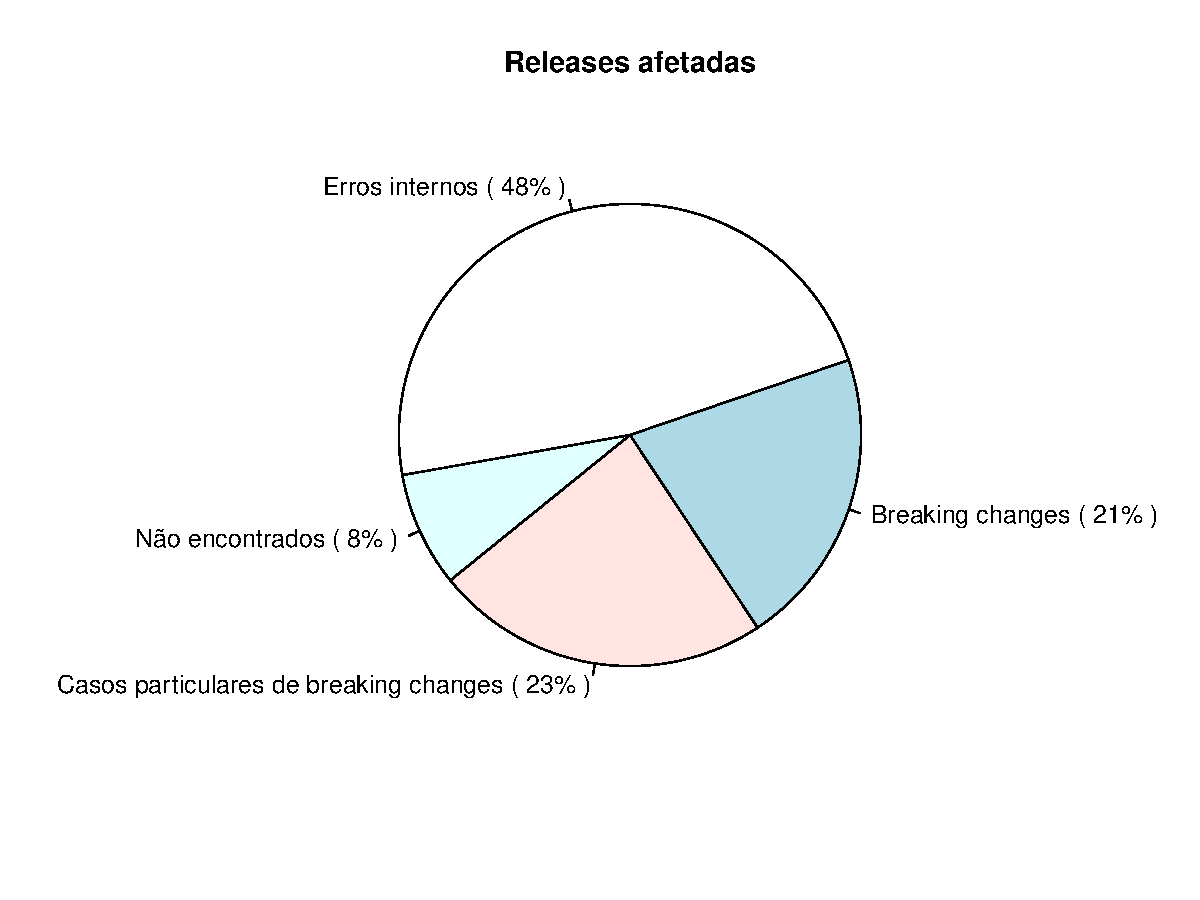
\includegraphics[scale=0.7]{figuras/pre_res_rq1.pdf}
    \caption{Resultado dos casos de erros em função das \textit{releases}}
    \label{fig:pre_res_rq1}
\end{figure}{}

\section{QP2. Como os provedores introduzem \textit{breaking changes} em uma \textit{release}}
\label{res:qp2}

\subsubsection{\textbf{Classificação das \textit{Breaking changes}}}

Ao todo, foram 43 casos de \textit{breaking changes} distribuídas em 39 clientes. Todos esses casos foram agrupados em 8 diferentes categorias das quais se encaixavam. A Tabela \ref{tab:bc_category} apresenta cada uma dessas categorias, bem como a quantidade de clientes e a quantidade de \textit{releases} que cada categoria atingiu.

\begin{table}[]
\begin{tabular}{|l|c|c|c|c|}
\hline
\centering
\textbf{Categoria}           & \textbf{Pacotes afetados} & \textbf{\%}   & \textbf{\textit{Release} afetadas} & \textbf{\%}    \\ \hline
Alteração de regras          & 12              & 27,9 & 64                          & 33,68 \\
Provedores incompatíveis     & 8               & 18,6 & 30                          & 15,78 \\
Alteração de tipo de objeto  & 8               & 18,6 & 24                          & 12,63 \\
Objeto indefinido            & 4               & 9,3  & 25                          & 13,15 \\
Código errado                & 4               & 9,3  & 13                          & 6,84  \\
Código não-atualizado        & 3               & 6,97 & 25                          & 13,15  \\
Renomeação de função         & 3               & 6,97 & 5                           & 2,63  \\
Arquivo não encontrado       & 1               & 2,32 & 4                           & 2,1  \\ \hline
\textbf{Total}               & 43              &      & 190                         &       \\ \hline
\end{tabular}
\caption{Categorias dos casos de \textit{breaking change}}
\label{tab:bc_category}
\end{table}

A seguir, encontra-se uma descrição sobre cada categoria.

\begin{itemize}
    \item \textbf{Alteração de regras}: este caso foi o principal que impactou os clientes. Essa categoria contém os casos de \textit{breaking change} no qual os provedores possuíam um determinado comportamento, mas alteraram algumas de suas regras/funcionalidades e impactaram os seus clientes. Não foi uma simples alteração no código, tal como uma alteração de tipo de variáveis, ou um código escrito de maneira errada, mas sim uma regra no qual o cliente tinha como sólida, foi alterada; %Por exemplo, o pacote \textit{request@2.18.0} introduziu uma alteração em seu código\footnote{https://github.com/request/request/commit/d05b6ba72702c2411b4627d4d89190a5f2aba562\#diff-168726dbe96b3ce427e7fedce31bb0bcR857}, como pode ser visto na Figura \ref{fig:bc_category_change_rule_1}.

    %\begin{figure} \centering 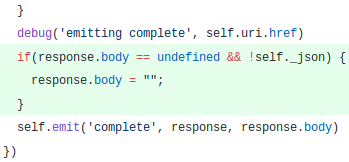
\includegraphics[scale=0.6]{figuras/bc_category_change_rule_1.png} \caption{Alteração de regra de funcionamento do \textit{request}} \label{fig:bc_category_change_rule_1} \end{figure}{}

    %Nesse caso, o \textit{request} adiciona uma \textit{string} vazia ao invés de manter \textit{undefined} o corpo de uma requisição. Esse caso do \textit{request} ocorreu exatamente como foi explicado por \citeonline{Foo:2018:ESC:3236024.3275535} dizendo que os pacotes evoluem independentemente dos clientes. Essa alteração na regra do \textit{request} reflete em uma evolução do pacote, mas o cliente não esperava essa alteração e confiava que o corpo da resposta fosse retornado como \textit{undefined} em caso de erro, por isso o cliente quebrou.

    \item \textbf{Provedores incompatíveis}: nessa categoria, há um provedor direto A e um provedor indireto B envolvido, o qual alterou o seu código, o que não gerou um erro, mas provocou no provedor A um comportamento inesperado, ou seja, o provedor B passou a ser incompatível com o provedor A. Nessa categoria, nenhum dos provedores contém um erro, mas sim uma incompatibilidade; %Um exemplo disso ocorreu com os pacotes \textit{babel-eslint}\footnote{https://www.npmjs.com/package/babel-eslint} e \textit{escope}\footnote{https://www.npmjs.com/package/escope}, entretanto, o pacote \textit{escope} é um provedor indireto do \textit{babel-eslint}.

    %\begin{figure} \centering 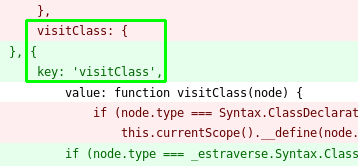
\includegraphics[scale=0.5]{figuras/bc_category_incompatibles_providers.png} \caption{Alteração de código do \textit{escope}} \label{fig:bc_category_incompatibles_providers} \end{figure}{}

    %A \textit{releases escope@3.4} realizou uma alteração no seu código, de acordo com a Figura \ref{fig:bc_category_incompatibles_providers}, mas que não reflete em um erro. Essa alteração impactou diretamente o pacote \textit{babel-eslint}, mesmo o pacote \textit{escope} não sendo um provedor direto do \textit{babel-eslint} e não ter introduzido um erro\footnote{https://github.com/estools/escope/issues/99\#issuecomment-178151491}. Com isso, há uma incompatibilidade entre os provedores e essa incompatibilidade precisou ser corrigida pelo \textit{babel-eslint} e não pelo \textit{escope}. Essa foi a \textit{breaking change} que mais surgiu na análise manual pois, dos 43 casos, 5 (11.6\%) refletiam essa incompatibilidade, uma vez que o \textit{babel-eslint} é provedor de 5.8\% de toda a base de dados.

    \item \textbf{Alteração de tipo de objeto}: essa é uma categoria de \textit{breaking changes} facilmente detectável em linguagens fortemente tipadas, mas no \textit{Javascript} representam um tipo de \textit{breaking change} que, por muitas vezes, pode nem afetar o código do cliente. Mas, neste trabalho, foram detectados 8 (18.6\%) de casos nos quais os provedores alteraram o tipo de alguma variável;

    %\begin{figure} \centering 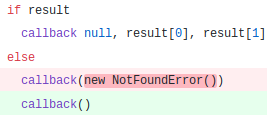
\includegraphics[scale=0.5]{figuras/bc_category_change_type.png} \caption{Alteração de um tipo \textit{array} para \textit{object}} \label{fig:bc_category_change_type} \end{figure}{}

    %Na Figura \ref{fig:bc_category_change_type} o provedor \textit{socket.io}\footnote{https://www.npmjs.com/package/socket.io} alterou alguns \textit{arrays} para \textit{object}\footnote{https://github.com/socketio/socket.io/commit/b73d9bea4efb48277eee685763026ff2df5a79ab}. Anteriormente, os clientes iteravam nesses \textit{arrays}, mas após essa alteração, os clientes foram afetados.

    \item \textbf{Objeto indefinido}: por vezes, os códigos podem estar todos corretos, mas então o provedor tenta acessar uma variável que não existe. Essa categoria de \textit{breaking change} representa os casos no qual os provedores tentaram obter acesso à alguma variável/objeto, mas que não existiam. Esses erros são os que facilmente podem ser consertados/evitados apenas adicionando o código da Listagem \ref{cod:undefined_object}:

    \begin{lstlisting}[style=bash, label=cod:undefined_object]
    this.var = this.var || {};
    \end{lstlisting}

    %Esse tipo de erro surgiu no pacote \textit{ember-cli-htmlbars-inline-precompile}\footnote{https://www.npmjs.com/package/ember-cli-htmlbars-inline-precompile}, no qual o desenvolvedor tenta acessar uma variável que não estava disponível. Mas, assim como o desenvolvedor já havia feito com as demais variáveis da Figura \ref{fig:bc_category_undefined_object}, uma simples alteração no código foi o suficiente.

    %\begin{figure} \centering 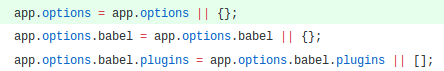
\includegraphics[scale=0.7]{figuras/bc_category_undefined_object.png} \caption{Correção do erro de objeto indefinido} \label{fig:bc_category_undefined_object} \end{figure}{}

    \item \textbf{Código errado}: este caso de \textit{breaking change} ocorreu quando o provedor escreveu um código semanticamente incorreto, gerando um erro na sua execução e afetando o cliente. Em linguagens compilada, esse tipo de erro seria facilmente identificado pelo compilador em tempo de compilação; %Foi exatamente isso que a dependência fez. Ao alterar o seu código, o desenvolvedor escreveu duas vezes a mesma variável, como pode ser visto na Figura \ref{fig:bc_category_wrong_code}. Assim como os erros do tipo \textit{undefined object}, os erros dessa categoria  são facilmente corrigidos.

    %\begin{figure} \centering 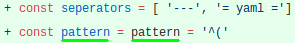
\includegraphics[scale=0.8]{figuras/bc_category_wrong_code.png} \caption{Código semanticamente incorreto} \label{fig:bc_category_wrong_code} \end{figure}{}

    \item \textbf{Código não-atualizado}: as \textit{breaking changes} desta categoria são as que o provedor atualiza o \textit{range} de seu provedor mas não altera o seu código para adaptar-se a ele. Assim, o erro está no primeiro provedor que contém um código desatualizado;

    \item \textbf{Renomeação de função}: as \textit{breaking changes} relacionadas à esta categoria foram facilmente detectáveis. Quando a mensagem de erro do \textit{node.js} era exibida como \textit{TypeError: var is not a function}, com pouca investigação já era possível identificar que uma determinada função não estava mais disponível, ou seja, havia sido removida ou alterado o seu nome; e

    %\begin{figure} \centering 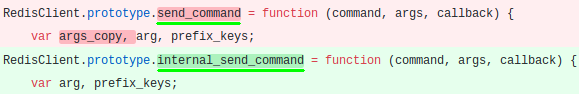
\includegraphics[scale=0.6]{figuras/bc_category_renamed_function.png} \caption{Alteração do nome de função} \label{fig:bc_category_renamed_function} \end{figure}{}

    \item \textbf{Arquivo não encontrado}: os casos de \textit{breaking change} relacionados à esta categoria são aqueles no qual o desenvolvedor realiza um acesso a um arquivo, mas esse não existe. O arquivo requerido pode não existir ou não estar disponível, uma vez que, referenciado no arquivo \textit{.npmignore} -- arquivo utilizado pelo \textit{npm} para ignorar arquivos durante o processo de publicação --, o arquivo existe mas não está disponível, mas também o arquivo pode não existir. Entretanto, o único caso de arquivo não encontrado ocorreu pois o arquivo \textit{index.js} estava referenciado no \textit{.gitignore}.% O provedor \textit{esprima-extract-comments}\footnote{https://www.npmjs.com/package/esprima-extract-comments} utilizava como provedor um \textit{fork} do pacote \textit{esprima}\footnote{https://github.com/ariya/esprima/} e o referencia em seu  \textit{package.json} para ser descarregado diretamente do \textit{Github}\footnote{https://github.com/jonschlinkert/esprima-extract-comments/blob/6b65a0f52f85bc6fa830d44e352ec3da9e9ef620/package.json\#L47}. Entretanto, o \textit{index.js} desse \textit{fork}, foi referenciado no \textit{.gitignore} e não estava disponível quando o \textit{npm} descarregou o pacote diretamente do \textit{Github}, mas o arquivo estava disponível se o pacote \textit{exprima} fosse descarregado diretamente do \textit{npm}.

\end{itemize}{} % Esse capítulo e nome é apenas uma sugestão.
\chapter{Cronograma de Atividades}
\label{cap:cronograma}

Nesta seção são apresentadas as atividades a serem desenvolvidas para a execução da proposta. O cronograma de realização das tarefas é apresentado na Tabela~\ref{tab:cronograma}.

\begin{enumerate}
\item \textbf{Documentação da Ferramenta \textit{BCDetect}}
    \begin{enumerate}
        \item Traduzir a documentação da \textit{BCDetect} para o inglês.
    \end{enumerate}{}
\item \textbf{Análise dos dados da RQ3.}
    \begin{itemize}
        \item Agrupar as ações dos clientes para se recuperarem das \textit{breaking changes}; e
        \item Analisar o tempo que as \textit{breaking changes} levaram para serem consertadas.
    \end{itemize}{}
\item \textbf{Análise dos Resultados.}
    \begin{itemize}
        \item Completar os resultados da QP1; e
        \item Completar os resultados da QP2.
    \end{itemize}{}
\item \textbf{Escrita do TCC 2.}
\item \textbf{Entrega do TCC 2.}
\item \textbf{Apresentação do TCC 2.}
\end{enumerate}

\begin{table}[h!]
\centering
\renewcommand{\arraystretch}{1.3}
\caption{Cronograma de atividades}
\label{tab:cronograma}
\scalefont{0.9}
\begin{tabular}{|c|c|c|c|c|c|}
\hline
\multirow{2}{*}{\textbf{Atividade}} & \multicolumn{2}{l|}{\textbf{2019}} & \multicolumn{3}{l|}{\textbf{2020}} \\ \cline{2-6} 
             & Nov & Dez & Jan & Fev & Mar \\ \hline
\textbf{1}   &  X  &     &     &     &     \\ \hline
\textbf{2}   &  X  &  X  &     &     &     \\ \hline
\textbf{3}   &  X  &  X  &     &     &     \\ \hline
\textbf{4}   &     &  X  &  X  &  X  &     \\ \hline
\textbf{5}   &     &     &     &     &  X  \\ \hline
\textbf{6}   &     &     &     &     &  X  \\ \hline
\end{tabular}
\end{table} % Esse capítulo e nome é apenas uma sugestão.

% Apendices.
%\appendix
%\chapter{Instalação de Ferramentas}
\label{ape:instalacao:ferramentas}

Os apêndices são usados para disponibilizar materiais extras que por questões de espaço ou estilo de escrita não foram colocados diretamente no texto. Por exemplo, \textit{scripts}, instruções de instalação das ferramentas utilizadas pelo trabalho, partes de código fonte e questionários que tenham sido aplicados, tabelas com resultados...

(ATENÇÃO - veja com o seu orientador se é necessário disponibilizar algum material extra sobre algum capítulo em anexo!)



%bibliografia
\bibliographystyle{abntex2-alf}
\bibliography{main} % geração automática das referências a partir do arquivo main.bib

\backmatter
\end{document}
